% ---------------------------------------------------------------------------
% Author guideline and sample document for EG publication using LaTeX2e input
% D.Fellner, v1.13, Nov 13, 2007

\documentclass{egpubl}
\usepackage{egsgp15}

% --- for  Annual CONFERENCE
% \ConferenceSubmission % uncomment for Conference submission
% \ConferencePaper      % uncomment for (final) Conference Paper
% \STAR                 % uncomment for STAR contribution
% \Tutorial             % uncomment for Tutorial contribution
% \ShortPresentation    % uncomment for (final) Short Conference Presentation
%
% --- for  CGF Journal
% \JournalSubmission    % uncomment for submission to Computer Graphics Forum
% \JournalPaper         % uncomment for final version of Journal Paper
%
% --- for  CGF Journal: special issue
% \SpecialIssueSubmission    % uncomment for submission to Computer Graphics Forum, special issue
\SpecialIssuePaper         % uncomment for final version of Journal Paper, special issue
%
% --- for  EG Workshop Proceedings
% \WsSubmission    % uncomment for submission to EG Workshop
% \WsPaper         % uncomment for final version of EG Workshop contribution
%
 \electronicVersion % can be used both for the printed and electronic version

% !! *please* don't change anything above
% !! unless you REALLY know what you are doing
% ------------------------------------------------------------------------

% for including postscript figures
% mind: package option 'draft' will replace PS figure by a filname within a frame
\ifpdf \usepackage[pdftex]{graphicx} \pdfcompresslevel=9
\else \usepackage[dvips]{graphicx} \fi

\PrintedOrElectronic

% prepare for electronic version of your document
\usepackage{t1enc,dfadobe}

\usepackage{egweblnk}
\usepackage{cite}

% For backwards compatibility to old LaTeX type font selection.
% Uncomment if your document adheres to LaTeX2e recommendations.
% \let\rm=\rmfamily    \let\sf=\sffamily    \let\tt=\ttfamily
% \let\it=\itshape     \let\sl=\slshape     \let\sc=\scshape
% \let\bf=\bfseries

% end of prologue

\usepackage{epstopdf}
\usepackage[scaled=.92]{helvet}
\usepackage{amsmath}
\usepackage{url}
%\newcommand{\comment}[1]{}

\usepackage{times}

%% Inline URLs
\usepackage{url}

%% AMS mathematics packages
\usepackage{amsfonts,amsmath,amssymb}

%% The 'graphicx' package allows for the inclusion of EPS figures.
\usepackage{graphicx}

%% use this for zero \parindent and non-zero \parskip, intelligently.

\usepackage{parskip}

%% For cells spanning multiple rows or columns in tables
\usepackage{multirow}

% this package allows psgrag (replace text in eps figures, adapt it to the paper style)
\usepackage{psfrag}


%% Arrays
%\usepackage{array}

%% A tabular column that left-aligns its contents with a ragged-right margin (p{} justifies by default). Requires array.
%\newcolumntype{x}[1]{%
%>{\raggedright\hspace{0pt}}p{#1}}%

% This package allows multi-line comments.
\usepackage{verbatim}

%% Optional: the 'caption' package provides a nicer-looking replacement
%% for the standard caption environment. With 'labelfont=bf,'textfont=it',
%% caption labels are bold and caption text is italic.
%\usepackage[labelfont=bf,textfont=it]{caption}
%% Figures and tables with subfigures and subtables
%\usepackage[font=normalsize]{subcaption}

%% The `hyperref' package creates hyperlinked references and citations
%%
%% The package has a bug which may generate the following error message:
%%   ! pdfTeX error (ext4): \pdfendlink ended up in different nesting level than \pdfstartlink.
%% if a single citation is broken across pages. To debug, add the "draft"
%% option to hyperref, locate the offending citation, and change document
%% spacing a bit until the break is removed.
%%
%\usepackage[usenames,dvipsnames]{xcolor}% for hyperref
%\usepackage[citecolor=black,citebordercolor=white,colorlinks=false]{hyperref}

% Text wrapping around figure
\usepackage{wrapfig}

% In-para lists
\usepackage{paralist}

% Formatting the list environments
\usepackage{enumitem}
\setdescription{leftmargin=0.25cm}

% text colors
\usepackage[usenames,dvipsnames]{color}

% algorithm package
\usepackage[]{algorithm2e}


% list
\newenvironment{my_itemize}{
\begin{description} %{labelitemi}{$\bullet$}
  \setlength{\itemsep}{1pt}
  \setlength{\parskip}{0pt}
  \setlength{\parsep}{0pt}
  }
{\end{description}}

\newcounter{mycounter}
\newenvironment{noindlist}
 {\begin{list}{\arabic{mycounter}.~~}{\usecounter{mycounter} \labelsep=0em \labelwidth=0em \leftmargin=0em \itemindent=0em}}
 {\end{list}}

%% Symbols
\newcommand{\ba}{\mathbf{a}}
\newcommand{\bb}{\mathbf{b}}
\newcommand{\bc}{\mathbf{c}}
\newcommand{\bd}{\mathbf{d}}
\newcommand{\be}{\mathbf{e}}
\newcommand{\bff}{\mathbf{f}}
\newcommand{\bg}{\mathbf{g}}
\newcommand{\bh}{\mathbf{h}}
\newcommand{\bi}{\mathbf{i}}
\newcommand{\bj}{\mathbf{j}}
\newcommand{\bk}{\mathbf{k}}
\newcommand{\bl}{\mathbf{l}}
\newcommand{\bm}{\mathbf{m}}
\newcommand{\bn}{\mathbf{n}}
\newcommand{\bo}{\mathbf{o}}
\newcommand{\bp}{\mathbf{p}}
\newcommand{\bq}{\mathbf{q}}
\newcommand{\br}{\mathbf{r}}
\newcommand{\bs}{\mathbf{s}}
\newcommand{\bt}{\mathbf{t}}
\newcommand{\bu}{\mathbf{u}}
\newcommand{\bv}{\mathbf{v}}
\newcommand{\bw}{\mathbf{w}}
\newcommand{\bx}{\mathbf{x}}
\newcommand{\by}{\mathbf{y}}
\newcommand{\bz}{\mathbf{z}}
\newcommand{\bA}{\mathbf{A}}
\newcommand{\bB}{\mathbf{B}}
\newcommand{\bC}{\mathbf{C}}
\newcommand{\bD}{\mathbf{D}}
\newcommand{\bE}{\mathbf{E}}
\newcommand{\bF}{\mathbf{F}}
\newcommand{\bG}{\mathbf{G}}
\newcommand{\bH}{\mathbf{H}}
\newcommand{\bI}{\mathbf{I}}
\newcommand{\bJ}{\mathbf{J}}
\newcommand{\bK}{\mathbf{K}}
\newcommand{\bL}{\mathbf{L}}
\newcommand{\bM}{\mathbf{M}}
\newcommand{\bN}{\mathbf{N}}
\newcommand{\bO}{\mathbf{O}}
\newcommand{\bP}{\mathbf{P}}
\newcommand{\bQ}{\mathbf{Q}}
\newcommand{\bR}{\mathbf{R}}
\newcommand{\bS}{\mathbf{S}}
\newcommand{\bT}{\mathbf{T}}
\newcommand{\bU}{\mathbf{U}}
\newcommand{\bV}{\mathbf{V}}
\newcommand{\bW}{\mathbf{W}}
\newcommand{\bX}{\mathbf{X}}
\newcommand{\bY}{\mathbf{Y}}
\newcommand{\bZ}{\mathbf{Z}}
\newcommand{\balpha}{\mbox{\boldmath$\alpha$}}
\newcommand{\bgamma}{\mbox{\boldmath$\gamma$}}
\newcommand{\bGamma}{\mbox{\boldmath$\Gamma$}}
\newcommand{\bmu}{\mbox{\boldmath$\mu$}}
\newcommand{\bphi}{\mbox{\boldmath$\phi$}}
\newcommand{\bksi}{\mbox{\boldmath$\xi$}}
\newcommand{\bPhi}{\mbox{\boldmath$\Phi$}}
\newcommand{\bSigma}{\mbox{\boldmath$\Sigma$}}
\newcommand{\bsigma}{\mbox{\boldmath$\sigma$}}
\newcommand{\btheta}{\mbox{\boldmath$\theta$}}

\newcommand{\Ex}{\mathbb{E}}
\newcommand{\Var}{\mathbb{V}ar}

\newcommand{\mB}{\mathcal{B}}
\newcommand{\mL}{\mathcal{L}}
\newcommand{\mN}{\mathcal{N}}
\newcommand{\mU}{\mathcal{U}}
\newcommand{\mC}{\mathcal{C}}
\newcommand{\mS}{\mathcal{S}}
\newcommand{\mR}{\mathcal{R}}
\newcommand{\mD}{\mathcal{D}}
\newcommand{\mT}{\mathcal{T}}
\newcommand{\mV}{\mathcal{V}}
\newcommand{\mSl}{\mathcal{S}_l}
\newcommand{\mNl}{\mathcal{N}_l}
\newcommand{\mDll}{\mathcal{D}_{l,l'}}

\def\ll{{\mathcal{\ell}}}

\def\A{{\cal A}}
\def\B{{\cal B}}
\def\C{{\cal C}}
\def\D{{\cal D}}
\def\E{{\cal E}}
\def\F{{\cal F}}
\def\G{{\cal G}}
\def\H{{\cal H}}
\def\I{{\cal I}}
\def\J{{\cal J}}
\def\K{{\cal K}}
\def\L{{\cal L}}
\def\M{{\cal M}}
\def\N{{\cal N}}
\def\O{{\cal O}}
\def\P{{\cal P}}
\def\Q{{\cal Q}}
\def\R{{\cal R}}
\def\S{{\cal S}}
\def\T{{\cal T}}
\def\U{{\cal U}}
\def\V{{\cal V}}
\def\W{{\cal W}}
\def\X{{\cal X}}
\def\Y{{\cal Y}}
\def\Z{{\cal Z}}
\def\Re{{\mathbb R}}
\def\Cx{{\mathbb C}}
\def\Ze{{\mathbb Z}}
\def\Na{{\mathbb N}}
\def\Wh{{\mathbb W}}
\def\bd{\partial}
\def\ud{\mathrm{d}}
\def\eps{\varepsilon}
\def\dist{\textrm{dist}}
\DeclareMathOperator*{\argmax}{arg\,max}

%%%%%%%%%%%%%%%%%%%%%%%%%%%%%%%%%%%%%%%%%%%%%%%%%%%%%%%%%%%%%%%%%%%
%%%%%%%%%%%%%%%%%%%%%%% 4. COMMENTS %%%%%%%%%%%%%%%%%%%%%%%%%%%%%%%
%%%%%%%%%%%%%%%%%%%%%%%%%%%%%%%%%%%%%%%%%%%%%%%%%%%%%%%%%%%%%%%%%%%

%% Inlined comments
\def\marrow{}
\def\vangelis#1{\marrow\textcolor{magenta}{({Vangelis says: }{#1})}}
%\def\vangelis#1{}
\def\haibin#1{\marrow\textcolor{green}{({Haibin says: }{#1})}}

%\def\rev#1{\marrow\textcolor{red}{{#1}}}
\def\rev#1{#1}


%%%%%%%%%%%%%%%%%%%%%%%%%%%%%%%%%%%%%%%%%%%%%%%%%%%%%%%%%%%%%%%%%%%
%%%%%%%%%%%%%%%%%%%%% 5. SPACE COMPRESSION %%%%%%%%%%%%%%%%%%%%%%%%
%%%%%%%%%%%%%%%%%%%%%%%%%%%%%%%%%%%%%%%%%%%%%%%%%%%%%%%%%%%%%%%%%%%

\linespread{0.9}





\setlength{\skip\footins}{0.3cm}

% ---------------------------------------------------------------------
% EG author guidelines plus sample file for EG publication using LaTeX2e input
% D.Fellner, v1.17, Sep 23, 2010


\title[Analysis and synthesis of 3D shape families\\ via deep-learned generative models of surfaces]%
      {Analysis and synthesis of 3D shape families\\ via deep-learned generative models of surfaces}

% for anonymous conference submission please enter your SUBMISSION ID
% instead of the author's name (and leave the affiliation blank) !!
\author[H. Huang \& E. Kalogerakis \& B. Marlin]
       {Haibin Huang
        \,\,\,\,\,\,\,\,\,\,\,\,\,\,\,\,\,\,\,\,\,\,\,\,\,\,\,\,\,
        Evangelos Kalogerakis
        \,\,\,\,\,\,\,\,\,\,\,\,\,\,\,\,\,\,\,\,\,\,\,\,\,\,\,\,\,
        Benjamin Marlin \\
        University of Massachusetts Amherst\\
       }


% ------------------------------------------------------------------------

% if the Editors-in-Chief have given you the data, you may uncomment
% the following five lines and insert it here
%
% \volume{27}   % the volume in which the issue will be published;
% \issue{1}     % the issue number of the publication
% \pStartPage{1}      % set starting page


%-------------------------------------------------------------------------


\begin{document}

 \teaser{
 \centering
\vskip -12mm
 \includegraphics[width=0.95\textwidth]{figures/teaser.pdf}
\vskip -2mm
\caption{Given a collection of 3D shapes, we train a probabilistic model that performs joint shape analysis and synthesis.
 (Left) Semantic parts and corresponding points on shapes inferred by our model. (Right) New shapes synthesized by our model.}
\label{fig:teaser}
}

\maketitle

\begin{abstract}
\rev{We present a method for joint analysis and synthesis of geometrically diverse\ 3D\ shape families.  Our method first learns part-based templates such that an optimal set of fuzzy point and part correspondences is computed between the shapes of an input collection based on a probabilistic deformation model. In contrast to previous template-based approaches, the geometry and deformation parameters of our part-based templates are learned from scratch. Based on the estimated shape correspondence, our method also learns a probabilistic generative model  that hierarchically captures statistical relationships of corresponding surface point positions and parts as well as their existence in the input shapes. A deep learning procedure is used to capture these hierarchical relationships. The resulting generative model is used to produce control point arrangements that drive shape synthesis by combining and deforming parts from the input collection. The generative model also yields compact shape descriptors that are used to perform fine-grained classification.  Finally, it can be also coupled with the probabilistic deformation model to further improve shape correspondence. We provide qualitative and quantitative
evaluations of our method for  shape correspondence, segmentation, fine-grained classification and synthesis. Our experiments  demonstrate superior correspondence and segmentation results  than previous state-of-the-art approaches.} 


\begin{classification} % according to http://www.acm.org/class/1998/
\CCScat{Computer Graphics}{I.3.5}{Computational Geometry and Object Modeling}
\end{classification}

\end{abstract}

%%%%%%%%%%%%%%%%%%%%%%%%%%%%%%%%%%%%%%%%%%%%%%%%%%%%%%%%%%%%%%%%%%%%%%%%
% Introduction
%%%%%%%%%%%%%%%%%%%%%%%%%%%%%%%%%%%%%%%%%%%%%%%%%%%%%%%%%%%%%%%%%%%%%%%%

\section{Introduction}
\label{sec:intro}

\vspace{-2mm}

Discovering geometric and semantic relationships of 3D shapes is fundamental to several computer graphics applications. In particular, several tools for geometric modeling, manufacturing, shape retrieval and exploration can benefit from algorithms that automatically extract part, region and point correspondences within large shape collections. During the recent years, due to the growing number of online 3D shape repositories (Trimble Warehouse, Turbosquid and so on), a number of algorithms have been proposed to jointly analyze shapes in large collections to discover such correspondences. The key advantage of these algorithms is that they do not treat shapes in complete isolation from each other, but rather extract useful mappings and correlations between shapes to produce results that are closer to what a human would expect. 

Although there has been significant progress on analysis of shapes with similar structure (e.g., human bodies) and similar types of deformations (e.g, isometries or near-isometries), dealing with collections of structurally and geometrically diverse shape families (e.g., furniture, vehicles) still remains an open problem. A promising approach to handle such collections is to iteratively compute part or/and point correspondences and existence using part-based or local non-rigid alignment \cite{Kim13,Huang13}. The rationale for such approach is that part correspondences can help localize point correspondences and improve local alignment, point correspondences can refine segmentations and local alignment, and in turn more accurate local alignment can further refine segmentations and point correspondences. One of the drawbacks of existing methods following this approach is that strict point-to-point correspondences are not that suitable for collections of shapes whose parts exhibit significant geometric variability, such as airplanes, bikes and so on. In addition, these methods use templates made out of basic primitives (e.g., boxes in \cite{Kim13}) or other mediating shapes \cite{Huang13}, whose geometry may drastically differ from the surface geometry of several shapes in the collection leading to inaccurate correspondences. In the case of template fitting, approximate statistics on the used primitives can be used to penalize unlikely alignments (e.g., Gaussian distributions on box positions and scales). However, these statistics capture rather limited information about the actual surface variability in the shapes of the input collection. \rev{Similarly, in the context of shape synthesis, shape variability is often modeled with statistics over predefined part descriptors that cannot be directly mapped back to surfaces \cite{Kalogerakis12} or parameters of simple basic primitives, such as boxes \cite{Fish14,Averkiou14}}.

\rev{We present a method that analyzes and synthesizes 3D shape collections by learning representations of surface variability from scratch. Our method has two main components: a probabilistic deformation model and a generative  surface model. The probabilistic deformation model jointly estimates fuzzy point correspondences and part segmentations of shapes through learned part-based templates. In contrast to previous works that use simple geometric primitives or pre-existing shapes as templates, our method  learns the template geometry and deformations from the input collection. The deformation model provides input to our generative surface model that aims to learn geometric and structural relationships of parts and corresponding surface point positions. Following the concept of deep learning (or hierarchical learning) \cite{Bengio09} widely used in computer vision and natural language processing, the key idea of our generative model is to learn relationships in the surface data hierarchically: our model learns geometric arrangements of points within individual parts through a first layer of latent variables. Then it encodes  interactions between the latent variables of the first layer through a second layer of latent variables whose values correspond to relationships of surface arrangements across different parts. Subsequent layers mediate  higher-level relationships related to the overall shape geometry, semantic attributes and structure. The hierarchical architecture of our model is well-aligned with the compositional nature of shapes: shapes usually have a well-defined structure,      their structure is defined through parts, parts are made of patches and point arrangements with certain regularities.}
%The latent variables of our model may have certain interpretations: for example,  some latent variables of the first layer are associated with the shape of airplane wings or tailplanes (e.g., straight or delta-shaped wings). Variables of the second layer capture geometric relationships of airplane parts (e.g., swept wings usually co-occur with swept tailplanes). Variables of the third layer are related to  high-level airplane attributes (e.g. fighter jets or propeller aircraft types).

\rev{Our method  can jointly learn the probabilistic deformation model and the generative surface model leading to improved shape correspondence. In addition, the generative model can be sampled to generate plausible point-sampled surfaces that automatically drive shape synthesis. \ Finally, its uppermost layer produces a compact shape descriptor, or feature representation, that can be used to perform fine-grained classification (e.g., airplanes can be categorized to fighter jets, propeller aircraft,  unmanned aerial vehicles, and so on).}

%We note that our method is complementary to functional maps \cite{Ovsjanikov12,Huang14}. Our method infers probabilities over points and part correspondences, following the notion of fuzzy (soft) correspondences \cite{Kim12,Solomon12} that can be considered as special cases of functional maps. \rev{We believe that our method is also complementary to methods that employ cycle consistency constraints \cite{Huang12,Huang14} and human pose or functionality-related priors \cite{Kim14}.} These methods, including functional maps, can benefit from initial point or part correspondences that our method can provide. 

\textbf{Contributions.} The contribution of our work is two-fold. First, we provide a probabilistic deformation model that estimates fuzzy point and part correspondences within structurally and geometrically diverse shape families. The main difference with previous work is that our method learns the geometry and deformation parameters of templates within a fully probabilistic framework to optimally achieve these tasks instead of relying on fixed primitives or pre-existing shapes. \rev{Second, we introduce a deep-learned probabilistic generative model of 3D shape surfaces that can be used to further optimize shape correspondences, synthesize surface point arrangements, and produce  compact shape descriptors for fine-grained classification.  Both probabilistic models can be learned together leading to joint shape analysis and synthesis.} To the best of our knowledge, our method is the first to apply deep learning for training generative models of 3D\ shape surfaces. In contrast to previous work on generative probabilistic models that rely on highly structured databases (e.g., manually segmented shapes), our deep-learned model synthesizes shapes without or minimal human supervision. While previous generative models usually encode only high-level part and shape descriptors, our model directly encodes surface geometry and shape structure. Instead of mixing-and-matching parts from a database to synthesize shapes as frequently done in prior work, the sampled surface point arrangements of our model can be used to also deform the input collection parts to create more novel shape variations. 


%%%%%%%%%%%%%%%%%%%%%%%%%%%%%%%%%%%%%%%%%%%%%%%%%%%%%%%%%%%%%%%%%%%%%%%%
% Related work
%%%%%%%%%%%%%%%%%%%%%%%%%%%%%%%%%%%%%%%%%%%%%%%%%%%%%%%%%%%%%%%%%%%%%%%%

\vskip -3mm
\section{Related Work}
\label{sec:related_work}

Our method is related to prior work on data-driven methods for computing shape correspondences in collections with large geometric and structural variability, statistical models of shapes, and deep Boltzmann machines. We review the most relevant work in these areas. A complete review of previous research in shape correspondences and segmentation is out of the scope of this paper. We refer the reader to recent surveys in shape correspondences \cite{vanKaick11},  segmentation \cite{Theologou2015}, and structure-aware shape processing \cite{Mitra13}. 

\textbf{Data-driven shape correspondences.} Analyzing shapes jointly in a collection to extract useful geometric, structural and semantic relationships often yields significantly better results than analyzing isolated single shapes or pairs of shapes, especially for classes of shapes that exhibit large geometric variability. This has been demonstrated in previous data-driven methods for computing point-based and fuzzy correspondences \cite{Kim12,Huang12,Huang13,Huang13b}.  However, these methods do not leverage the part structure of the input shapes and do not learn a model of surface variability. As a result, these methods often do not generalize well to collections of shapes with significant structural diversity. \rev{A number of data-driven methods have been developed to segment shapes and effectively parse their structure \cite{Kalogerakis10,Huang11,Sidi11,Hu12,Wang12,Laga13,Xu2014,Zhige2014}.} However, these methods build correspondences only at a part level, thus cannot be used to find more fine-grained point or region correspondences within parts. Some of these methods require several training labeled segmentations \cite{Kalogerakis10,vanKaick11,Zhige2014} as input, or require users to interactively specify tens to hundreds of constraints \cite{Wang12}. 

Our work is closer to that of Kim et al.~\shortcite{Kim13}. Kim et al. proposed a method that estimates point-level correspondences, part segmentations, rigid shape alignments, and a statistical model of shape variability based on template fitting. The templates are made out of boxes that iteratively fit to segmented parts. Boxes are rather coarse shape representations and in general, shape parts frequently have drastically different geometry than boxes. Our method also makes use of templates to estimate correspondences and segmentations, however, their geometry and deformations are learned from scratch. Our produced templates are neither pre-existing parts nor primitives, but new learned parts equipped with probabilities over their point-based deformations. Kim et al.'s statistical model learns shape variability only in terms of individual box parameters (scale and position) and cannot be used for shape synthesis. In contrast, our statistical model encodes both shape structure and actual surface geometry, thus it can be used to generate shapes. Kim et al.'s method computes hard correspondences via closest points, which are less suitable for typical online shape repositories of inanimate objects. Our method instead infers probabilistic, or fuzzy, correspondences and segmentations via a probabilistic deformation model that combines non-rigid surface alignment, feature-based matching, as well as a deep-learned statistical model of surface geometry and shape structure.  

\textbf{Statistical models of 3D shapes.} Early works developed statistical models of shapes in specific domains, such as faces \cite{Blanz99}, human bodies \cite{Allen03}, and poses \cite{Anguelov05}. Yingze et al.~\shortcite{Yingze13} proposed a statistical model of sparse sets of anchor points by deforming a mean template shape using thin-plate spline (TPS) transformations for shapes, like cars, fruits, and keyboards. Our work can be seen as a generalization of these previous works to domains where shapes differ in both their structure and geometry and where no single template or mean shape can be used. 

A number of approaches have tried to model shape variability using Principal Component Analysis or Gaussian Process Latent Variable models on Signed Distance Function (SDF) representations of shapes \cite{Sandhu11:NKBPE,Chen11:SOPRU,Prisacariu11:SSS,Dame13}. However, the dimensionality of SDF voxel-based representations is very high, requiring the input shapes to be discretized at rather coarse voxel grids or use compression schemes that tend to eliminate surface features of the output shapes. Various ad-hoc weights are frequently used to infer coherent SDF values for the output shapes. \rev{Other methods use deformable templates made out of oriented boxes \cite{Ovsjanikov11,Kim13,Averkiou14}, and model shape variability in terms of the size and position of these boxes. Xu et al. \shortcite{Xu12} mixes-and-matches parts through set evolution with  part mutations (or deformations) following the  box parametrization approach of \cite{Ovsjanikov11} and part crossovers controlled by user-speficied fitness scores. Fish et al.~\shortcite{Fish14} and Yumer et al.~\shortcite{Yumer14} represent shapes in terms of multiple basic primitives (boxes, planes, cylinders etc) and capture shape variability in terms of primitive sizes, relative orientations, and translations. As a result, these methods do not capture statistical variability at the actual surface level and cannot directly be used to generate new surface point arrangements.} Kalogerakis et al.~\shortcite{Kalogerakis12} proposed a generative model of shape structure and part descriptors (e.g., curvature histograms, shape diameter, silhouette features). However, these descriptors are not invertible i.e., they cannot be directly mapped back to surface points. As a result, their model cannot be used to output surface geometry and was only used for shape synthesis by retrieving and recombining database parts without further modifications. \rev{In constrast to the above approaches, our generative model jointly analyzes and synthesizes 3D shape families, outputs both structure and actual surface geometry, as well as learned class-specific shape descriptors.}

\textbf{Deep Boltzmann Machines.} \rev{Our statistical model of surface variability follows the structure of a general class of  generative models, known as Deep Boltzmann Machines (DBMs) in the machine learning literature. DBMs have been used   for speech and image generation \cite{Ranzato11,Roux11,Mohamed12,Salakhutdinov12}, and can also be combined  with discriminative models \cite{Kae2013} for labeling tasks. In a concurrent work, Wu et al. \cite{Wu2015} proposed DBMs built over voxel representations of 3D shapes to produce generic shape descriptors and reconstruct low-resolution shapes from input depth maps.  Our model in inspired by prior work on DBMs to develop a deep generative model of 3D\ shape surfaces. Our model has several differences compared to previous DBM formulations. Our model aims at capturing continuous variability of surfaces instead of pixel or voxel interactions. To  capture surface variability, we use Beta distributions to model surface point locations instead of Gaussian or Bernoulli distributions often used in DBMs. In addition, the connectivity of layers in our model takes into account the structure of shapes based on their parts. Since shape collections have typically a much smaller size than image or audio collections, and since the geometry of surfaces tend to vary smoothly across neighboring points, we use spatial smoothness priors during training. We found that all these adaptations were important to generate surface geometry. }

\vskip -2mm




%%%%%%%%%%%%%%%%%%%%%%%%%%%%%%%%%%%%%%%%%%%%%%%%%%%%%%%%%%%%%%%%%%%%%%%%
% Overview
%%%%%%%%%%%%%%%%%%%%%%%%%%%%%%%%%%%%%%%%%%%%%%%%%%%%%%%%%%%%%%%%%%%%%%%%

\vskip -3mm
\section{Overview}
\label{sec:overview}

Given a 3D model collection representative of a shape family, our goal is to compute probabilistic point correspondences and part segmentations of the input shapes (Figure \ref{fig:teaser}, left), as well as learn a generative model of 3D shape surfaces (Figure \ref{fig:teaser}, right). At the heart of our method lies a probabilistic deformation model that learns \rev{part templates} and uses them to compute fuzzy point correspondences and segmentations. We now provide an overview of our \rev{part template learning} concept, our probabilistic deformation model, and our generative surface model. 

\textbf{Learned part templates.} Our method computes probabilistic surface correspondences by learning suitable \rev{part templates} from the input collection. As \rev{part template}, we denote a learned arrangement of surface points that can be optimally deformed towards corresponding parts of the input shapes under a probabilistic deformation model. To account for structural differences in the shapes of the input collection, the \rev{part templates} are learned with a hierarchical procedure. Our method first clusters the input collection into groups containing structurally similar shapes, such as benches, four-legged chairs and office chairs (Figure \ref{fig:hierarchy}c). Then a \rev{template} for each semantic part per cluster is learned (Figure \ref{fig:hierarchy}b). Given the learned group-specific \rev{part templates}, our method learns higher-level \rev{templates} for semantic parts that are common across different groups e.g. seats, backs, legs, armrests in chairs (Figure \ref{fig:hierarchy}a). The top-level \rev{part templates} allow our method to establish correspondences between shapes that belong to structurally different groups, yet share parts under the same label. If parts are unique to a group (e.g., office chair bases), we simply transfer them to the top level and do not establish correspondences to incompatible parts with different label coming from other clusters.

\begin{figure}[t]
\centering
\includegraphics[width=1.0\columnwidth]{figures/hierarchy_learn}
\vskip -2mm
\caption{Hierarchical \rev{part template} learning for a collection of chairs. (a) Learned high-level \rev{part templates} for all chairs. (b) Learned \rev{part templates} per chair type or group (benches, four-legged chairs, office chairs). (c) Representative shapes per group and exemplar segmented shapes (in red box). }
\vskip -8mm
\label{fig:hierarchy}
\end{figure}

\textbf{Probabilistic deformation model.} At the heart of our algorithm lies a probabilistic deformation model (Section \ref{sec:part_representation_learning}). The model evaluates the probability of deformations applied on the \rev{part templates} under different corresponding point and part assignments over the input shape surfaces. By performing probabilistic inference on this model, our method iteratively computes the most likely deformation of the \rev{part templates} to match the input shape parts (Figure \ref{fig:deformation}). At each iteration, our method deforms the \rev{part templates}, and updates probabilities of point and part assignments over the input shape surfaces. The updated probabilistic point and part assignments iteratively guides the deformation and vice versa until convergence.

\textbf{Generative surface model.} Based on the estimated probability distributions over corresponding point and part assignments on all the input shapes of the collection, our method learns a probabilistic model characterizing the structural and surface variability within a shape family (Section \ref{sec:bsm}). The surface variability is encoded in the model through a joint probability distribution that captures relationships between parts and surface point locations within the shape family. For example, consider airplanes. The position of wingtips is strongly related to the positions of other points on the same wing (i.e., the overall wing geometry), as well as the part arrangement and surface geometry of the whole airplane. These complex relationships of points and parts in the shapes of a family are hierarchically captured through latent variables. The model contains a layer of latent variables whose assignments are associated with arrangements of surface points within the same part. Higher-level layers of latent variables progressively capture relationships between surface points belonging to different shape parts. The latent variables also capture dominant modes of surface point arrangements corresponding to structurally different shape groups. By sampling the latent variables on the top layer, our model can generate parts and surface points that are used to synthesize new shapes. \rev{The top layer also produces shape descriptors that can be used for fine-grained classification.} Through the captured relationships between point locations, the model can be used to further improve correspondences in the shapes of the collection. 

\textbf{Pre-processing.} Our method requires the following pre-processing, or initialization: first, we rely on the rigid alignments provided by Kim et al. \shortcite{Kim13} to consistently orient the input shapes of each collection. Practically, we found that our surface variability model can tolerate incorrectly aligned shapes in the collections (e.g. about 5\% of the input shapes were not aligned correctly in the dataset it was trained on). Second, our method requires as input a labeled segmentation for at least one shape per group (Figure \ref{fig:hierarchy}c, red boxes). The segmentation can be provided by either the user, or an automatic co-segmentation technique. In the case of manual input, to facilitate the user, our method automatically clusters the shapes into groups and selects an exemplar shape per group. The user is asked to segment these exemplar shapes. In the case of co-segmented input, we use the segmentations provided by Kim et al. \shortcite{Kim13}. We note that the provided segmentations are used for initialization only: given initial segments, our methods learns the \rev{part templates} and improves the shape segmentations. 



%%%%%%%%%%%%%%%%%%%%%%%%%%%%%%%%%%%%%%%%%%%%%%%%%%%%%%%%%%%%%%%%%%%%%%%%
% Deformation Model
%%%%%%%%%%%%%%%%%%%%%%%%%%%%%%%%%%%%%%%%%%%%%%%%%%%%%%%%%%%%%%%%%%%%%%%%

\vskip -3mm
\section{Probabilistic deformation model}
\label{sec:part_representation_learning}

Our method takes as input a collection of shapes, and outputs groups of structurally similar shapes together with learned \rev{part templates} per group (Figure \ref{fig:hierarchy}). Given the group-specific \rev{part templates}, our method also outputs high-level \rev{part templates} for the whole collection. A probabilistic model is used to infer the \rev{part templates}. The model evaluates the joint probability of hypothesized \rev{part templates}, deformations of these \rev{templates} towards the input shapes, as well as shape correspondences and segmentations. The probabilistic model is defined over the following set of random variables:
\begin{description}[leftmargin=1em]
\setlength{\itemsep}{4pt}
\setlength{\parskip}{0pt}
\setlength{\parsep}{0pt}
\item[Part templates] $\bY = \{\bY_k\}$ where $\bY_k \in  \mathbb{R}^3$ denotes the 3D position of a point $k$ on a latent \rev{part template}. There are total $K$ such variables, where $K$ is the  number of points on all \rev{part templates}. The number of points per \rev{part template} is determined from the provided exemplar shape parts. 
\item[Deformations] $\bD = \{\bD_{t,k}\}$ where $\bD_{t,k} \in \mathbb{R}^3$ represents the position of a point $k$ on a \rev{part template} as it deforms towards the shape $t$. Given $T$ input shapes and $K$ total points across all \rev{part templates}, there are  $K \cdot T$ such variables. 
\item[Point correspondences] $\bU = \{U_{t,p}\}$ where $U_{t,p} \in \{1,2,...,K\}$ represents the ``fuzzy'' correspondence of the surface point $p$ on an input shape $t$ with points on the \rev{part templates}. In our implementation, each input shape is uniformly sampled with $5000$ points, thus there are total  $5000 \cdot T$ such random variables. 
\item[Surface segmentation] $\bS = \{S_{t,p}\}$ where $S_{t,p} \in \{1,...,L\}$ represents the part label for a surface point $p$ on an input shape $t$. $L$ is the number of available \rev{part templates}, corresponding to the total number of semantic part labels. There are also $5000 \cdot T$ surface segmentation variables. 
\item[Input surface points] $\bX_t = \{ \bX_{t,p} \}$ where $X_{t,p} \in \mathbb{R}^3$ represents the 3D position of a surface sample point $p$ on an input shape $t$. 
\end{description}



\begin{figure}[t!]
\centering
\includegraphics[width=1.02\columnwidth]{figures/deformation_iteration}
%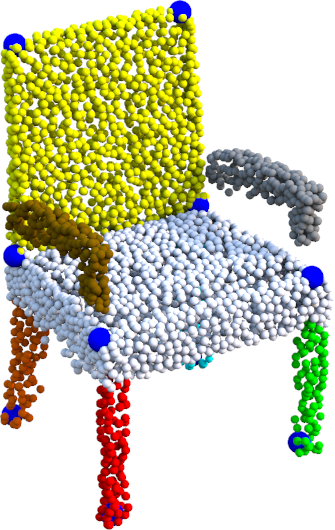
\includegraphics[width=0.24\columnwidth]{figures/deformation_learned}
%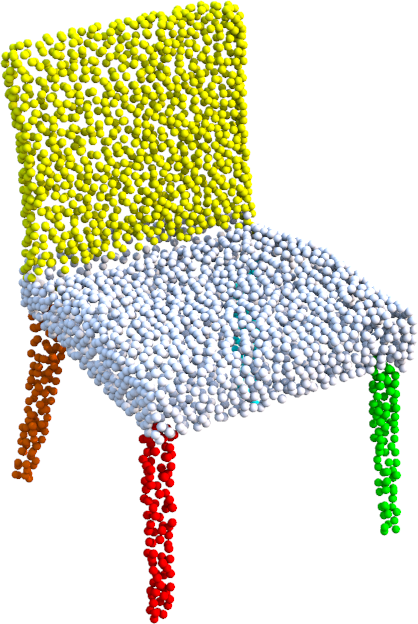
\includegraphics[width=0.24\columnwidth]{figures/deformation_def_0}
%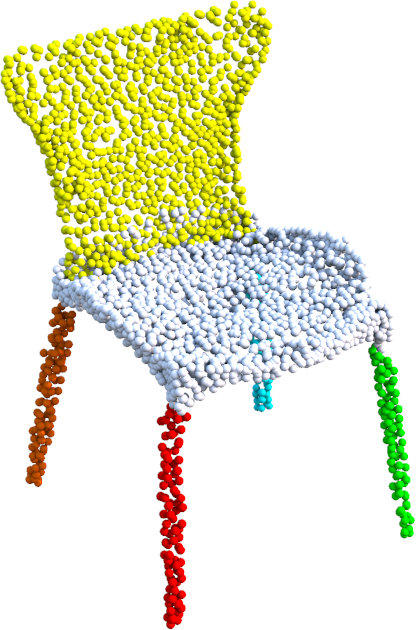
\includegraphics[width=0.24\columnwidth]{figures/deformation_def_1}
%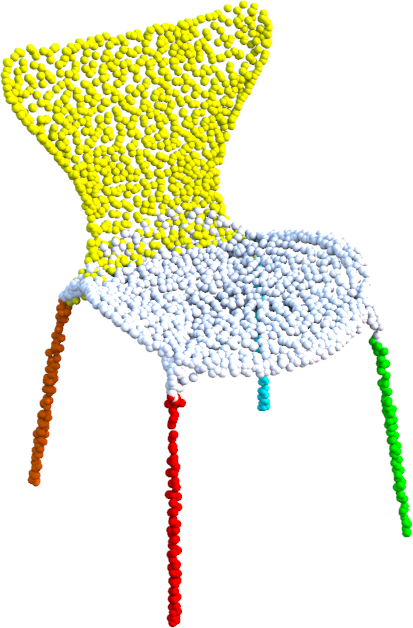
\includegraphics[width=0.24\columnwidth]{figures/deformation_def_2}
%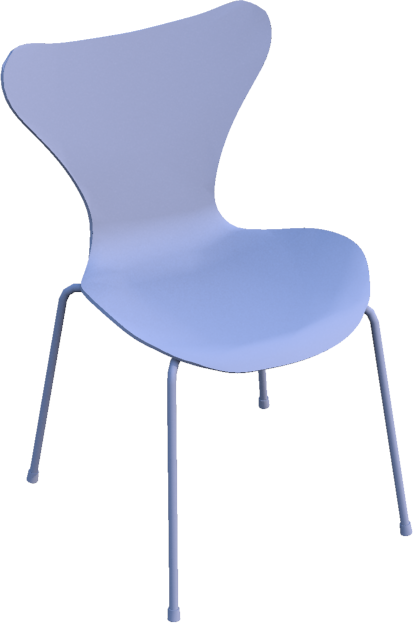
\includegraphics[width=0.24\columnwidth]{figures/deformation_target}
%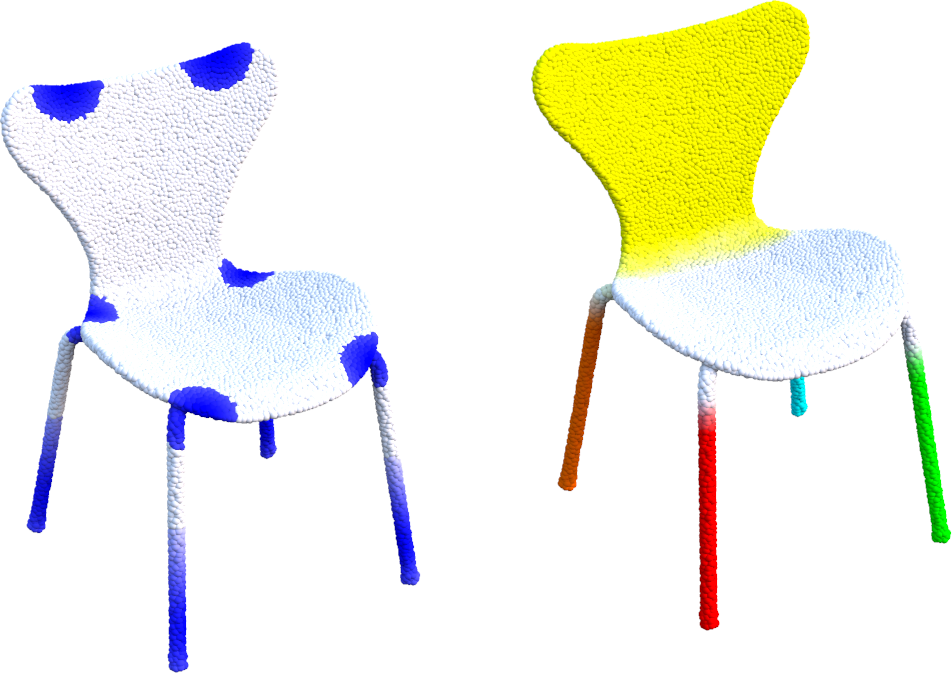
\includegraphics[width=0.24\columnwidth]{figures/deformation_seg_corr_0}
%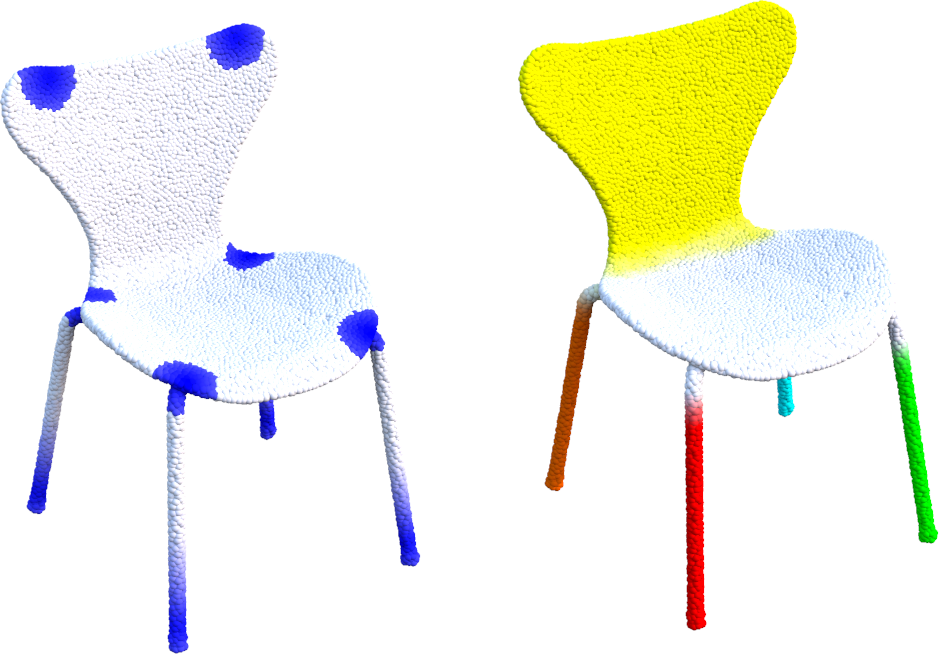
\includegraphics[width=0.24\columnwidth]{figures/deformation_seg_corr_1}
%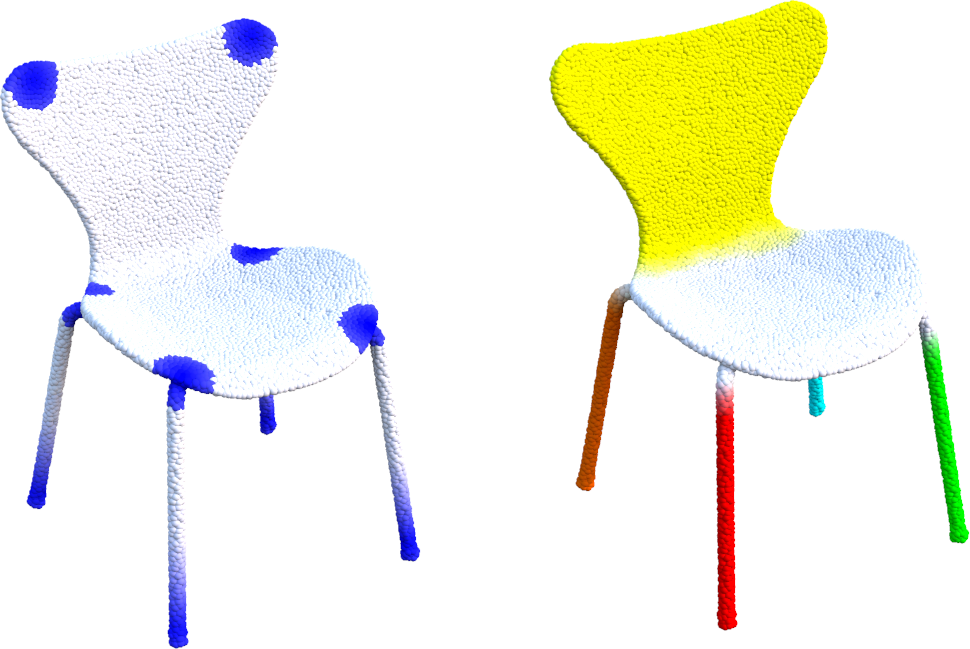
\includegraphics[width=0.24\columnwidth]{figures/deformation_seg_corr_2}
\vskip -2mm
\caption{Given learned \rev{part templates} for four-legged chairs, our method iteratively deforms them towards an input shape through probabilistic inference. At each iteration, probability distributions over deformations, point correspondences and segmentations are inferred according to our probabilistic model (probabilistic correspondences are shown only for the points appearing as blue spheres on the learned \rev{part templates}).}
\vskip -8mm
\label{fig:deformation}
\end{figure}


Our deformation model is defined through a set of factors, each representing the degree of compatibility of different assignments to the random variables it involves. The factors control the deformation of the \rev{part templates}, the smoothness of these deformations, the fuzzy point correspondences between each \rev{part template} and input shape, and the shape segmentations. The factors are designed out of intuition and experimentation. We now explain the factors used in our model in detail. 

\textbf{Unary deformation factor.} We first define a factor that assesses the consistency of deformations of individual surface points on the \rev{part templates} with an input shape. Given an input shape $t$ represented by its sampled surface points $\bX_t$, the factor is defined as follows:
\begin{align*}
& \phi_1 (\bD_{t,k}, \bX_{t,p}, U_{t,p} = k ) = \\
& \exp\bigg\{ -.5(\bD_{t,k} - \bX_{t,p})^T \Sigma_1^{-1} (\bD_{t,k} - \bX_{t,p}) \bigg\}
\end{align*} 
where the parameter $\Sigma_1$ is a diagonal covariance matrix estimated automatically, as we explain below. The factor encourages deformations of points on the \rev{part templates} towards the input shape points that are closest to them. 

\textbf{Deformation smoothness factor.} This factor encourages smoothness in the deformations of the \rev{part templates}. Given a pair of neighboring surface points $k, k'$ on an input \rev{template}, the factor is defined as follows:
\begin{align*}
& \phi_2( \bD_{t,k}, \bD_{t,k'}, \bY_k, \bY_{k'} ) = \\
& \exp\bigg\{ -.5( (\bD_{t,k} - \bD_{t,k'})- (\bY_k - \bY_{k'}) )^T \Sigma_2^{-1} \\ 
& \,\,\,\,\,\,\,\,\,\,\,\,\,\,\,\,\,\,\,\,\,\,\,\,\,\,\,\,\,((\bD_{t,k} - \bD_{t,k'})- (\bY_k - \bY_{k'})) \bigg\}
\end{align*}
The factor favors locations of deformed points relative to their deformed neighbors that are closer to the ones on the (undeformed) \rev{part templates}. The covariance matrix $\Sigma_2$ is diagonal and is also estimated automatically. In our implementation, we use the $20$ nearest neighbors of each point $k$ to define its neighborhood. 

\textbf{Correspondence factor.} This factor evaluates the compatibility of a point on a \rev{part template} with an input surface point by comparing their geometric descriptors:
\begin{align*}
& \phi_3 ( U_{t,p} = k, \bX_t ) = \exp\bigg\{ - .5(\bff_k - \bff_{t,p})^T \Sigma_3^{-1}(\bff_k -\bff_{t,p}) \bigg\}
\end{align*}
where $\bff_k$ and $\bff_{t,p}$ are geometric descriptors evaluated on the points of the \rev{part template} and the input surface $\bX_t$ respectively, $\Sigma_3$ is a diagonal covariance matrix. Our descriptor includes geometric information from shape diameter \cite{shapira2008consistent} (under three different normalizing parameters $\alpha=1,2,4$), average geodesic distance \cite{Hilaga01}, and PCA \cite{Kim13}, forming a $10-$ dimensional vector.

\textbf{Segmentation factor.} This factor assesses the consistency of each part label with an individual surface point on an input shape. The part label depends on the fuzzy correspondences of the point with each \rev{part template}: 
\begin{align*}
\phi_4 ( S_{t,p} = l, U_{t,p} = k ) =
\begin{cases}
    1,& \text{if } label(k) = l \\
    \epsilon,& \text{if } label(k) \ne l \\
\end{cases} 
\end{align*}
where $label(k)$ represents the label of the \rev{part template} with the point $k$. The constant $\epsilon$ is used to avoid numerical instabilities during inference, and is set to $10^{-3}$ in our implementation. 
 
\textbf{Segmentation smoothness.} This factor assesses the consistency of a pair of neighboring surface points on an input shape with part labels: 
\begin{align*}
\phi_5 ( S_{t,p} = l, S_{t,p'} = l', \bX_t ) = 
\begin{cases}
    1 - \Phi_{t,p,p'},& \text{if } l \ne l' \\
    \Phi_{t,p,p'},& \text{if } l = l' \\
\end{cases} 
\end{align*}
where $p'$ is a neighboring surface point to $p$ and:
\begin{align*}
\Phi_{t,p,p'} = \exp\bigg\{ - .5(\bff_{t,p} - \bff_{t,p'})^T \Sigma_5^{-1} (\bff_{t,p} - \bff_{t,p'})  \bigg\}
\end{align*}
To define the neighborhood for each point $p$, we first segment the input shape into convex patches based on the approximate convex segmentation algorithm \cite{Asafi13}. Then we find the $20$ nearest neighbors from the patch the point $p$ belongs to. The use of information from convex patches helped our method compute smoother boundaries between different parts of the input shapes. 

\textbf{Deformation model.} Our model is defined as a Conditional Random Field (CRF) \cite{Koller09} multiplying all the above factors together and normalizing the result to express a joint probability distribution over the above random variables. 

\begin{align}
& P_{crf}( \bY, \bU, \bS, \bD | \bX ) = \frac{1}{Z(\bX)} \prod\limits_t \bigg[ \prod\limits_{k,p} \phi_1 (\bD_{t,k}, \bX_{t,p}, U_{t,p}) \nonumber \\ 
& \cdot \prod\limits_{k, k'} \phi_2( \bD_{t,k}, \bD_{t,k'}, \bY_k, \bY_{k'} ) \cdot \prod\limits_{p} \phi_3 ( U_{t,p}, \bX_t ) \nonumber  \\
& \cdot \prod\limits_{p} \phi_4 ( S_{t,p}, U_{t,p} ) \cdot \prod\limits_{p, p'} \phi_5 ( S_{t,p}, S_{t,p'}, \bX_t ) \bigg]
\label{eq:objective}
\end{align}

\textbf{Mean-field inference.} Using the above model, our method infers probability distributions for \rev{part templates} and deformations, as well as shape segmentations and correspondences. To perform inference, we rely on the mean-field approximation theory due to its efficiency and guaranteed convergence properties. We approximate the original probability distribution $P_{crf}$ with another simpler distribution $Q$ such that the KL-divergence between these two distributions is minimized: 
\begin{align*}
P_{crf}( \bY, \bU, \bS, \bD | \bX )  \approx Q( \bY, \bU, \bS, \bD | \bX )
\end{align*}
where the approximating distribution $Q$ is a product of individual distributions associated with each variable:
\begin{align*}
& Q( \bY, \bU, \bS, \bD | \bX ) = \\
& \prod\limits_k Q( \bY_k ) \prod\limits_{t,k} Q( \bD_{t,k} ) \prod\limits_{t,p} Q( U_{t,p} ) \prod\limits_{t,p} Q( S_{t,p} )
\end{align*}

For continuous variables, we use Gaussians as approximating individual distributions, while for discrete variables, we use categorical distributions. We provide all the mean-field update derivations for each of the variables in the supplementary material. Learning the \rev{part templates} entails computing the expectations of \rev{part template} variables $\bY_k$ with respect to their approximating distribution $Q(\bY_k)$. For each \rev{part template} point $\bY_k$, the mean-field update is given by:

\begin{align*}
& Q(\bY_k) \propto \exp\bigg\{ -.5(\bY_k - \bmu_k )^T \Sigma_2^{-1} ( \bY_k -  \bmu_k )  \bigg\}
\end{align*}
where:
\begin{align*}
\bmu_k = \frac{1}{|\mN(k)|} \sum\limits_{k'} \big( \Ex_Q[\bY_{k'}] + \frac{1}{T}\sum\limits_t(\Ex_Q[\bD_{t,k}] - \Ex_Q[\bD_{t,k'}]) \big)
\end{align*}
and $\mN(k)$ includes all neighboring points $k'$ of point $k$ on the \rev{part template}. As seen in the above equation, to compute the mean-field updates, we need to compute expectations over deformations of \rev{part templates}. However, to compute these expectations, we require an initialization for the \rev{part templates}, as described next. 

\textbf{Clustering.} The first step of our method is to cluster the input shapes into groups of structurally similar shapes. For this purpose, we define a dissimilarity measure between two shapes based on our unary deformation factor. We measure the amount of deformation required to map the points of one shape towards the corresponding points of the other shape in terms of their Euclidean distance, and vice versa. 
%To compute the closest corresponding point for a query point, we only consider points whose normal has the same direction with the normal of the query point. 
For small datasets (with less than 100 shapes), we compute the dissimilarities between all-pairs of shapes, then use the affinity propagation clustering algorithm \cite{Frey07}. The affinity propagation algorithm takes as input dissimilarities between all pairs of shapes, and outputs a set of clusters together with a set of representative, or exemplar, shape per cluster. We note that another possibility would be to use all the factors of the model to define a dissimilarity measure, however, this proved to be computationally too expensive. For larger datasets, we compute a graph over the input shapes, where each node represents a shape, and edges connect shapes which are similar according to a shape descriptor \cite{Kim12}. We compute distances for pairs of shapes connected with an edge, then embed the shapes with the Isomap technique \cite{Tenenbaum:2000:GGF} in a $20$-dimensional space. We use the distances in the embedded space as dissimilarity metric for affinity propagation. 

As mentioned above, affinity propagation also identifies a representative, or exemplar, shape per cluster. In the case of manual initialization of our method, we ask the user to segment each identified exemplar shape per group, or let him select a different exemplar shape if desired. In the case of non-manual segmentation initialization, we rely on a co-segmentation technique to get an initial segmentation of each exemplar shape. In our implementation we use the co-segmentation results provided by Kim et al. \shortcite{Kim13}. Even if the initial segmentation of the exemplar shapes is approximate, our method updates and improves the segmentations for all shapes in the collection based on our probabilistic deformation model, as demonstrated in the results. To ensure that the identified exemplar shape has all (or most) representative parts per cluster in the case of automatic initialization, we modify the clustering algorithm to force it to select an exemplar from the shapes with the largest number of parts per cluster based on the initial shape co-segmentations. Figure \ref{fig:hierarchy} shows the detected clusters for a small chair dataset and user-specified shape segmentations for each exemplar shape per cluster. 

\textbf{Inference procedure and parameter learning.} Given the clusters and initially provided parts for exemplar shapes, the mean-field procedure follows the Algorithm \ref{algorithm}. At line 1, we initialize the approximating distributions for the \rev{part templates} according to a Gaussian centered at the position of the surface points on the provided exemplar parts. We then initialize the deformed versions of the \rev{part templates} using the provided exemplar parts after aligning them with each exemplar shape (lines 2-5). Alignment is done by finding the least-squares affine transformation that maps the exemplar shapes with the shapes of their group. The affine transformation is used to account for anisotropic scale differences between shapes in each group. We initialize the approximating distributions for correspondences and segmentations with uniform distributions (lines 6-9). Then we start an outer loop (line 10) during which we update the covariance matrices (line 11) and execute an inner loop for updating the approximating distributions for segmentations, correspondences and deformations for each input shape (lines 12-24). The covariance matrices are computed through piecewise training \cite{Sutton05} on each factor separately using maximum likelihood. We provide the parameter updates in the supplementary material. Finally, we update the distributions on \rev{part templates} (line 25). The outer loop for updating the \rev{part templates} and parameters requires $5-10$ iterations to reach convergence in our datasets. Convergence is checked based on how much the inferred point position on the \rev{part template} deviate on average from the ones of the previous iteration.  For the inner loop, we practically found that running more mean-field iterations ($10$ in our experiments) for updating the deformations helps the algorithm converge to better segmentations and correspondences. During the inference procedure, our method can infer negligible probability (below $10^{-3}$) for one or more part labels for all points on an input shape. This happens when an input shape has parts that are subset of the ones existing in its group. In this case, the \rev{part templates} missing from that shape are deactivated e.g., Figure \ref{fig:deformation} demonstrates this case where the input shape does not have armrests. 

\textbf{High-level part template learning.} Learning the \rev{part templates} at the top level of hierarchy follows the same algorithm as above with different input. Instead of the shapes in the collection, the algorithm here takes as input the learned \rev{part templates} per group. For initialization, we try each part from the lower level to initialize each higher-level \rev{part template} per label, and select the one with highest probability according to our model (Equation \ref{eq:objective}). The \rev{part templates}, deformations and correspondences are updated according to Algorithm \ref{algorithm}. For this step, we omit the updates for segmentations, since the algorithm works with individual parts. We note that it is straightforward to extend our method to handle more hierarchy levels of \rev{part templates} (e.g., splitting the clusters into sub-clusters also leading to the use of more exemplars per shape type, or group) by applying the same algorithm hierarchically and using a hierarchical version of affinity propagation \cite{Givoni11}. Experimentally, we did not see any significant benefit from using multiple exemplars per group at least in the datasets we used.



\begin{algorithm}
\LinesNumbered
\SetNlSty{texttt}{}{:}
\SetKwInOut{Input}{input}\SetKwInOut{Output}{output}
\Input{Input collection and initially segmented parts of exemplar shapes}
\Output{Learned \rev{part templates}, shape correspondences and segmentations}
\BlankLine

Initialize $\Ex_Q[\bY_k]$ from the position of the exemplar shape part points\;

\For{\textnormal{each shape} $t\leftarrow 1$ \KwTo $T$}
 {
  \For{\textnormal{each part template point} $k\leftarrow 1$ \KwTo $K$}
  {   
   Initialize $\Ex_Q[\bD_{t,k}]$ from the aligned part templates with the shape $t$\;
  }
  \For{\textnormal{each surface point} $p\leftarrow 1$ \KwTo $P$}
  {     
   Initialize $Q(U_{t,p})$ and $Q(S_{t,p})$ to uniform distributions\;
  }
 }
 
\Repeat{convergence}
{
  Update covariance matrices $\bSigma_1, \bSigma_2, \bSigma_3, \bSigma_5$;
        
  \Repeat{convergence}
  {     
        \For{\textnormal{each shape} $t\leftarrow 1$ \KwTo $T$}
         {  
            \For{\textnormal{each surface point} $p\leftarrow 1$ \KwTo $P$}
            { 
                  update correspondences $Q(\bU_{t,p})$\;
                  update segmentations $Q(\bS_{t,p})$\;
            }  
            \For{iteration $\leftarrow 1$ \KwTo $10$}
            { 
              \For{\textnormal{each part template point} $k\leftarrow 1$ \KwTo $K$}
                { 
                     update deformations $Q(\bD_{t,k})$;
                }
            }
         }
  }
  update part templates $Q(\bY)$\;
}
\vskip 1mm
\caption{Mean-field inference procedure.}
\label{algorithm}
\end{algorithm}






%%%%%%%%%%%%%%%%%%%%%%%%%%%%%%%%%%%%%%%%%%%%%%%%%%%%%%%%%%%%%%%%%%%%%%%%
% BSM Model
%%%%%%%%%%%%%%%%%%%%%%%%%%%%%%%%%%%%%%%%%%%%%%%%%%%%%%%%%%%%%%%%%%%%%%%%

\vskip -3mm
\section{Generative surface model}
\label{sec:bsm}

\begin{figure*}[t!]
\centering
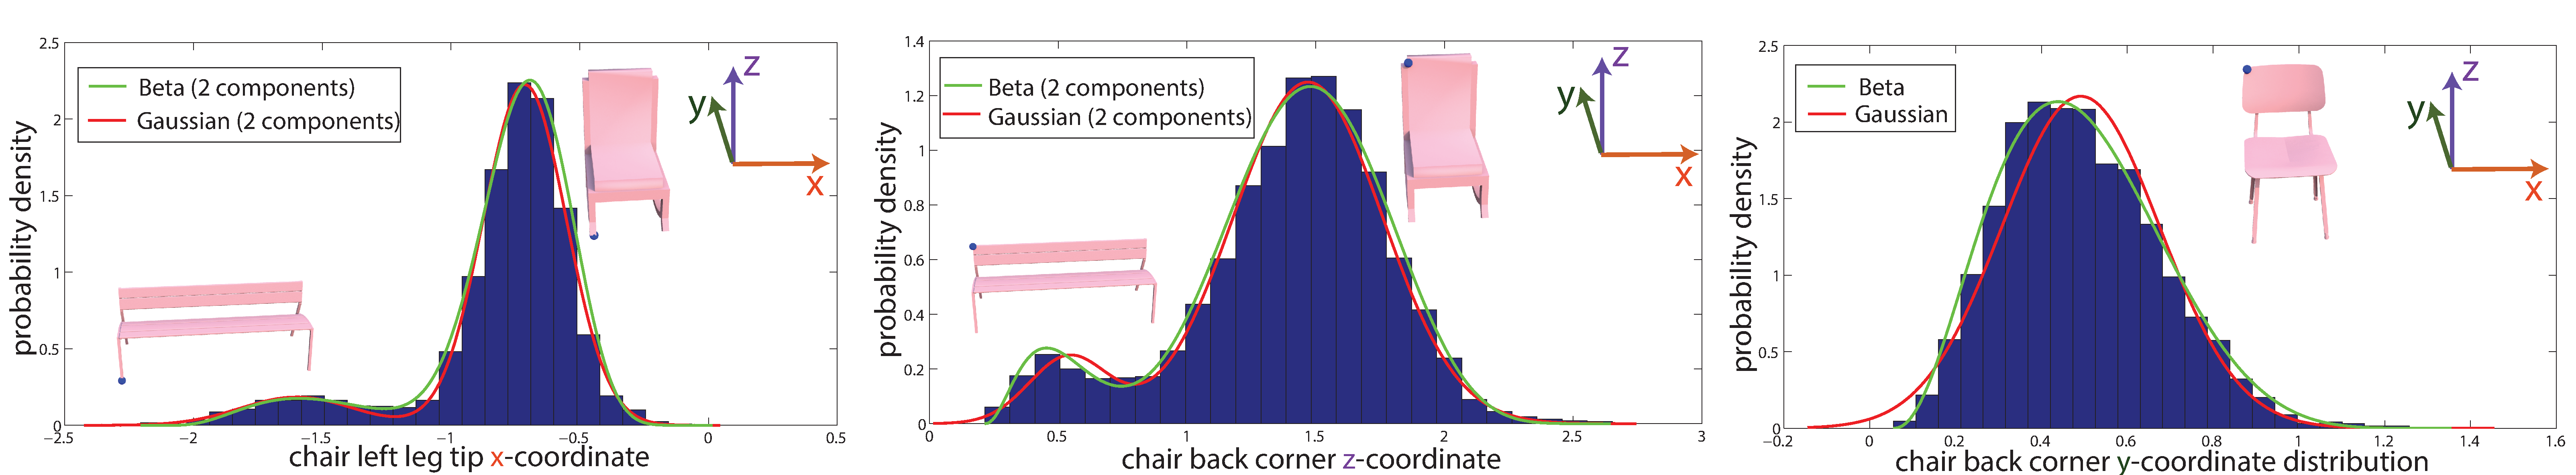
\includegraphics[width=0.95\textwidth]{figures/figure_histograms.pdf}
\vskip -2mm
\caption{Examples of feature point coordinate histograms for chairs and fitted distributions. The fitted Beta distributions are bounded by the minimum and maximum values of the coordinates and fit the underlying probability density more accurately.}
\vskip -8mm
\label{fig:motivation}
\end{figure*}


We now describe a generative probabilistic model whose goal is to characterize surface variability within a shape family. This model is built on the probabilistic shape correspondences and segmentations estimated with the technique described in the previous section. Learning a model that characterizes surface variability poses significant challenges. First, even if we consider individual corresponding surface points, there is no simple probability distribution that can model the variability in their position. For example, Figure \ref{fig:motivation} shows the distributions over coordinates of characteristic feature points across the shapes of four-legged chairs. The coordinates are expressed in an object-centered coordinate system whose origin is located on the chairs' center of mass. We observe that (a) the distributions are not unimodal (Figure \ref{fig:motivation}, left and middle), (b) the modes usually correspond to different types of chairs, such as benches or single-person chairs, and similar modes appear for different feature points (Figure \ref{fig:motivation}, left and middle), (c) even if the distributions appear to be unimodal, they might not be captured with commonly used symmetric distributions, such as Gaussians (red curves). For example, a Gaussian distribution would assign noticeable probability density for unrealistic chairs whose back would be aligned with the center of mass, or is in front of it (with respect to the frontal viewpoint used to display the chairs in the above figure). Furthermore, there are important correlations in the positions of different corresponding points that would need to be captured by the generative model: for example, benches are usually associated with wide seats, short backs, and legs placed on the seat corners. Another complication is that shapes vary in structure: for example, some chairs have armrests, while some others do not. The existence of parts depends on the overall type of chairs. Thus, a generative model needs to capture such structural relationships between parts, as well as capture the dependencies of point positions conditioned on the existence of these parts in the input shapes. Finally, even if our 3D shapes are parameterized with a relatively moderate number of consistently localized points (about $5000$ points), the dimensionality of our input data is still very large ($15000$), which also needs to be handled by the learning procedure of our generative model. \rev{Following the literature in deep learning, the key idea is to design the generative model such that it capture interactions in the surface data hierarchically through multiple layers of latent variables. We experimented with different numbers of hidden layers, and discuss performance differences in Section \ref{sec:results_applications}.} Our surface variability model is defined over the following set of random variables:
\begin{description}[leftmargin=1em]
\setlength{\itemsep}{4pt}
\setlength{\parskip}{0pt}
\setlength{\parsep}{0pt}
\item[Surface point positions] $\bD = \{\bD_{k}\}$ where $\bD_{k} \in \mathbb{R}^3$ represents the position of a consistently localized point $k$ on an input shape expressed in object-centered coordinates. During the training of our model, these random variables are observed by using the inference procedure of the previous section i.e., they are given by the \rev{part template} deformations per input shape. We note that we drop the shape index $t$ since this variable is common across all shapes for our generative model. 
\item[Surface point existences] $\bE = \{\bE_{k}\}$ where $\bE_{k} \in \{0,1\}$ represents whether a point $k$ exists on an input shape. These variables are also observed during training the model of surface variability. They are determined by the inference procedure of the previous section based on which \rev{part templates} were active or inactive per input shape. 
\item[Latent variables for geometry] $\bH = \{H_m^{(1)},H_n^{(2)},H_o^{(3)}\}$ encode relationships of surface point location coordinates at different hierarchical levels. The super-script is an index for the different hidden layers in our model. 
\item[Latent variables for structure] $\bG = \{G_r\}$ encode structural relationships of parts existence in shapes.
\end{description}

\textbf{Model structure.} The generative model is defined through factors that express the interaction degree between the above variables.  The choice of the factors was motivated by experimentation and empirical observations. We start our discussion with the factors involving the observed surface point position variables. Given that these are continuously values variables, one way to model the distribution over point positions would be to use Gaussian distributions. However, as shown in Figure \ref{fig:motivation}, a Gaussian may incorrectly capture the variability even for a single surface point position. Instead, we use Beta distributions that bound the range of values for a variable, and whose density function is more flexible. 
%\begin{wrapfigure}{l}{0.4\columnwidth}
%  \begin{center}
%  \vspace{-10pt}
%    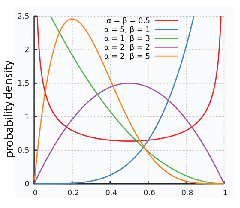
\includegraphics[width=0.5\columnwidth]{figures/beta.pdf}
%\vspace{-10pt}    
%  \end{center}
%\vspace{-10pt}  
%  \caption{Beta distributions}
%\vspace{-10pt}    
%  \label{fig:beta}
%\end{wrapfigure}
The Beta distribution over a single coordinate of an individual point location is defined as follows:
\begin{equation*}
P( D_{k,\tau} ) = \frac{1}{B} D_{k,\tau}^{a-1} \cdot (1 - D_{k,\tau})^{b-1}
\end{equation*}
where the index $\tau=1,2,3$ refers to the x-,y-, or z-coordinate of the point respectively, $B$ is a normalization factor, $a$, $b$ are positive-valued parameters that control the shape of the distribution. The distribution is defined over the interval $[0, 1]$, thus in our implementation we normalize all the observed coordinate values within this range. As discussed above, using a single distribution to capture the statistical variability of a point location is still inadequate since the point locations on a surface are not independent of each other. As shown in Figure \ref{fig:motivation}, the locations are multi-modal and modes are shared, thus we use latent variables to capture these common modes. Putting these empirical observations together, the interaction between point locations and latent variables can be modeled as follows: 
\begin{align*}
& \phi( \bD, \bH^{(1)}) = 
\nonumber \\
& \,\, \prod \limits_{k,\tau} D_{k,\tau}^{a_{k,\tau,0}-1} \cdot (1 - D_{k,\tau})^{b_{k,\tau,0}-1} 
\nonumber \\
& \cdot \prod \limits_{k,\tau} \prod\limits_{m \in \mN_k} D_{k,\tau}^{a_{k,\tau,m} H_m^{(1)}} \cdot (1 - D_{k,\tau})^{b_{k,\tau,m} H_m^{(1)}} 
\nonumber \\
& \cdot \prod \limits_{k,\tau} \prod\limits_{m \in \mN_k} D_{k,\tau}^{c_{k,\tau,m} (1-H_m^{(1)})} \cdot (1 - D_{k,\tau})^{d_{k,\tau,m} (1-H_m^{(1)})}
\end{align*}
where $a_{k,\tau,m}, b_{k,\tau,m},c_{k,\tau,m},d_{k,\tau,m}$ are positive weights expressing how strong is the interaction  between each latent variable $m$ with point $k$, $a_{k,\tau,0}, b_{k,\tau,0}$ are positive bias weights, $\mN_k$ denotes the subset of latent random variables of the first layer connected to the variable $D_k$. To decrease the number of parameters and enforce some sparsity in the model, we split the latent variables in the first layer into groups, where each group corresponds to a semantic part. We model the interaction between each point position with the first hidden layer variables that correspond to the semantic part it belongs to (see also Figure \ref{fig:graphical_model} for a graphical representation of our model). In this manner, each latent variable of the first layer can be thought of as performing a spatially sensitive convolution on the input points per part (see also supplementary material for the inference equations indicating this convolution).

As shown in Figure \ref{fig:motivation}, each group of shapes has its own distinctive parts e.g., benches are associated with wide and short backs. The latent variables of the second layer mediate the inter-dependencies of the part-level latent variables of the first layer. The choice of factors for those interactions are based on sigmoid functions that ``activate'' part-level geometry modes given certain global shape variability modes: 
\begin{align*}
\phi( \bH^{(1)}, \bH^{(2)} ) = \exp \bigg\{ \sum\limits_m w_{m, 0} H_m^{(1)} & + \sum\limits_{m,n} w_{m, n} H_m^{(1)} H_n^{(2)} \nonumber \\ 
& + \sum\limits_n w_{n, 0} H_n^{(2)} \bigg\}
\end{align*}
where the parameters $w_{m,n}$ control the amount of interaction between the latent variables of the first and second layer, $w_{m, 0}$, $w_{n, 0}$ are bias weights. Given the above factor, it can be seen that each latent variable is activated through sigmoid functions:
\begin{align*}
P( H_m^{(1)} = 1 | \bH^{(2)} ) = \sigma ( w_{m, 0} + \sum\limits_{n} w_{m, n} H_n^{(2)} ) \\
P( H_n^{(2)} = 1 | \bH^{(1)} ) = \sigma ( w_{n, 0} + \sum\limits_{m} w_{m, n} H_m^{(1)} ) 
\end{align*}
where $\sigma(x)=1/(1+exp(-x))$ represents the sigmoid function. 


\begin{figure}[t!]
\includegraphics[width=1.0\columnwidth]{figures/dbm}
\vskip -2mm
\caption{Graphical representation of the surface variability model based on our airplane dataset.}
\label{fig:graphical_model}
\vskip -8mm
\end{figure}


We model the interactions of the latent variables of the subsequent hidden layers in the same manner.  By multiplying all of the above factors, we combine them into a single probability distribution, which has the form of a deep Boltzmann machine \cite{Salakhutdinov12}. By taking into account that some factors must be deactivated when parts are non-existing in shapes (i.e., when the existence variables for their points are $0$), our final probability distribution has the following form: 
\begin{align}
& P_{bsm}( \bD, \bH, \bG, \bE ) = \frac{1}{Z} \exp \bigg\{ 
\nonumber  \\
& \sum\limits_{k,\tau} (a_{k,\tau,0}-1) \ln(D_{k,\tau})E_k + \sum\limits_{k,\tau} (b_{k,\tau,0}-1) \ln(1-D_{k,\tau})E_k 
\nonumber  \\
& +\sum\limits_{k,\tau,m \in \mN_k} a_{k,\tau,m} \ln(D_{k,\tau}) H_m^{(1)}E_k 
\nonumber  \\
& +\sum\limits_{k,\tau,m \in \mN_k} b_{k,\tau,m} \ln(1-D_{k,\tau}) H_m^{(1)}E_k
\nonumber  \\
& +\sum\limits_{k,\tau,m \in \mN_k} c_{k,\tau,m} \ln(D_{k,\tau}) (1-H_m^{(1)})E_k 
\nonumber  \\
& +\sum\limits_{k,\tau,m \in \mN_k} d_{k,\tau,m} \ln(1-D_{k,\tau}) (1-H_m^{(1)})E_k
\nonumber \\
& +\sum\limits_m w_{m, 0} H_m^{(1)} + \sum\limits_{m,n} w_{m, n} H_m^{(1)} H_n^{(2)} + \sum\limits_n w_{n,0}H_n^{(2)}
\nonumber \\
& + \sum\limits_{n,o} w_{n, o} H_n^{(2)} H_o^{(3)} + \sum\limits_o w_{o, 0} H_o^{(3)} 
\nonumber \\
& +\sum\limits_k w_{k,0} E_k + \sum\limits_{k,r} w_{k, r} E_k G_r + \sum\limits_r w_{r, 0}G_r \bigg\} 
\label{eq:BSM}
\end{align}
where $Z$ is a normalization constant. In the following paragraphs, we refer to this model as Beta Shape Machine (BSM) due to the use of Beta distributions to model  surface data.

\textbf{Parameter learning.} Learning  the parameters of the BSM model poses a number of challenges. Exact maximum likelihood estimation of the parameters is intractable in Deep Boltzmann machines, thus we resort to an approximate learning scheme, called contrastive divergence \cite{Koller09}. Contrastive divergence aims at maximizing the probability gap between the surface data of the input shapes and samples randomly generated by our model. The intuition is that by increasing the probability of the observed data relative to the probability of random samples, the parameters are tuned to model the input data better. The objective function of contrastive divergence is defined as follows: 
\begin{align*}
L_{CD} = \frac{1}{T} \sum\limits_t [ \ln \tilde{P}_{bsm}(\bksi_t) - \ln \tilde{P}_{bsm}(\bksi'_t) ]
\end{align*}
where $T$ is the number of training examples, $\tilde{P}_{bsm}$ is given by Equation \ref{eq:BSM} without the normalization factor $Z$ (known as unnormalized measure), $\bksi_t$ is an assignment to the variables of the model given an input shape $t$ and $\bksi'_t$ is an assignment to the variables according to a sample perturbed from the same input shape $t$. The assignments to the variables $E_k$ and $\bD_k$ per input shape $t$ are set by checking if the \rev{part template} exists in the input shape and finding the closest surface point to each point $k$ on the deformed \rev{part templates} for it respectively. The assignments for the latent variables are computed by performing mean-field inference and using the expectations of their approximating distributions, following Salakhutdinov et al. \cite{Salakhutdinov12} (see supplementary material for more details). The perturbed sample is generated by inferring the approximating probability distribution of the top-layer binary variables given an input shape, then sampling these binary variables according to their distribution, and finally computing the expectations of the approximating distributions of all the other variables in the model given the sampled values of the top layer. 


\begin{figure}[t!]
\centering
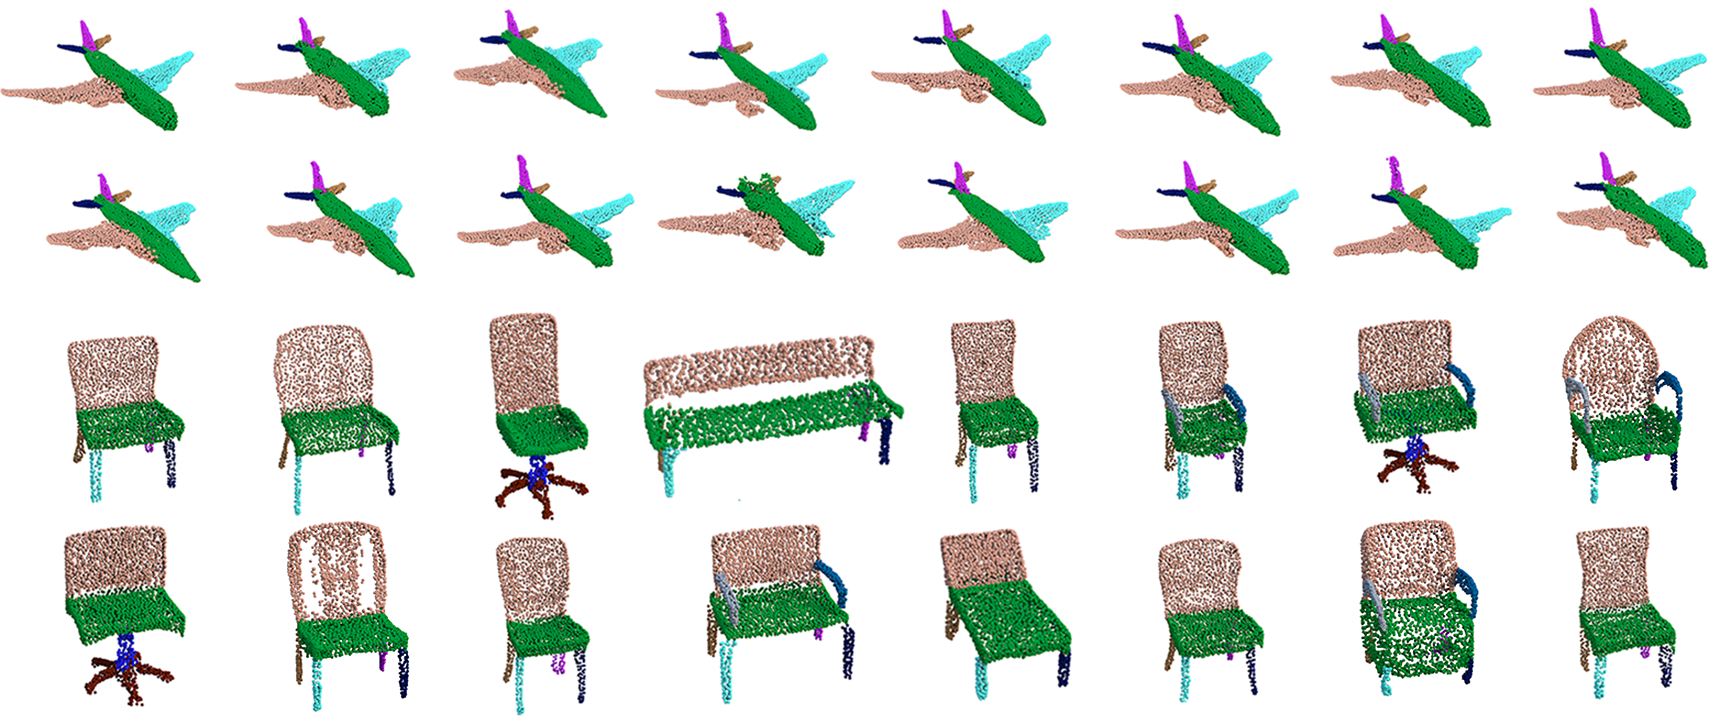
\includegraphics[width=0.99\columnwidth]{figures/bsm_sample}
\vskip -2mm
\caption{Samples generated from the BSM for airplanes and chairs. The generated shapes are implicitly segmented into labeled parts since each point is colored according to the label of the \rev{part template} it originated from.}
\vskip -8mm
\label{fig:sample_BSM}
\end{figure}


An additional complication in parameter learning is that even for collections whose shapes are parameterized with a relatively moderate number of points and even with the sparsity in the connections between the observed variables and the first hidden layer, the number of parameters ranges from $5$ to $10$ million. Yet the available organized 3D shape collections are limited in size e.g., the corrections we used contain only a few thousand shapes. A key idea in our learning approach is to use strong spatial priors that favor similar weights on the variables representing point positions that are spatially close to each other on average across the input shapes of our collections. To favor spatial smoothness in the learned parameters, we change the above objective function with the following spatial priors and $L^1$ norm regularization terms. The $L^1$ norm was desired to eliminate weak hidden node associations causing higher noise when sampling the model and also prevent model overfitting. The new objective function is defined as follows:
\begin{align*}
L_{CD,spatial} & = \frac{1}{T} \sum\limits_t [ \ln \tilde{P}_{bsm}(\bksi_t) - \ln \tilde{P}_{bsm}(\bksi'_t) ] 
\nonumber \\
& - \lambda_1 \sum\limits_{k,\tau,k' \in \mN_k,m} | a_{k,\tau,m} - a_{k',\tau,m} | - \lambda_2 \sum\limits_{k,\tau,m} | a_{k,\tau,m} | 
\nonumber \\
& - \lambda_1 \sum\limits_{k,\tau,k' \in \mN_k,m} | b_{k,\tau,m} - b_{k',\tau,m} | - \lambda_2 \sum\limits_{k,\tau,m} | b_{k,\tau,m} | 
\nonumber \\
& - \lambda_1 \sum\limits_{k,\tau,k' \in \mN_k,m} | c_{k,\tau,m} - c_{k',\tau,m} | - \lambda_2 \sum\limits_{k,\tau,m} | c_{k,\tau,m} | 
\nonumber \\
& - \lambda_1 \sum\limits_{k,\tau,k' \in \mN_k,m} | d_{k,\tau,m} - d_{k',\tau,m} | - \lambda_2 \sum\limits_{k,\tau,m} | d_{k,\tau,m} | 
\nonumber \\
& - \lambda_1 \sum\limits_{k,r,k' \in \mN_k} | w_{k,r} - w_{k',r} | 
\nonumber \\
& - \lambda_2( \sum\limits_{m,n} | w_{m,n} | - \sum\limits_{n,o} | w_{n,o} | - \sum\limits_{k,r} | w_{k,r} | ) \\
\end{align*}
where $\lambda_1, \lambda_2$ are regularization parameters, set to $10^{-3}$ and $10^{-4}$ respectively in our experiments, $\mN(k)$ here denotes all the variables representing point positions whose average distance to point $k$ is less than $10\%$ of the largest distance between a pair of points across all shapes. We perform projected gradient ascent to maximize the above objective function under the constraint that the parameters $a_{k,m}, b_{k,m},c_{k,m},d_{k,m}$ are all positive. The same parameters are initialized to random positive numbers according to a uniform distribution on $[10^{-7},10^{-3}]$, while the rest of the weights are initialized according to a normal distribution with mean $0$ and variance $0.1$. 

\begin{figure}[t!]
\centering
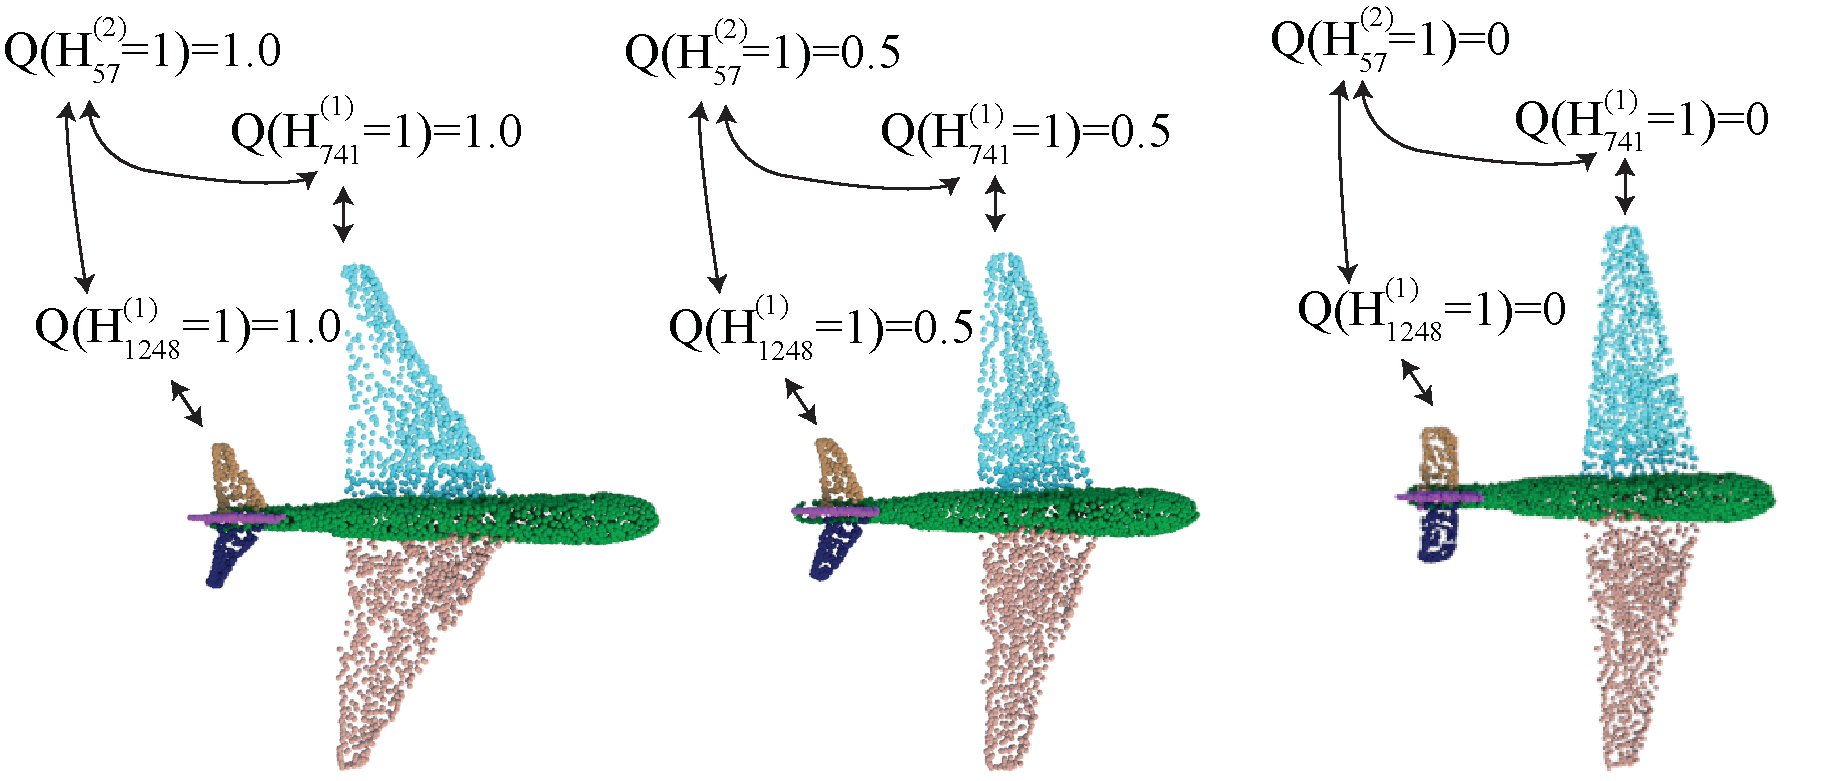
\includegraphics[width=0.9\columnwidth]{figures/motivation/motivation.pdf}
\vskip -3mm
\caption{\rev{Certain latent variables in our learned model have meaningful interpretations.  For example, given the leftmost delta-shaped wing arrangement, certain hidden variables of the first layer are activated (i.e., activation probability based on mean-field inference becomes approximately one), while given the rightmost straight wing arrangement, the same variables are deactivated. Similarly, other first layer variables are activated and deactivated  for triangular and straight tailplanes respectively. The model also learns that there is a potential statistical correlation between straight wings and tailplanes through variables of the second layer. Initializing the synthesis procedure with interpolated probabilities (e.g., 50\%) of these variables generate plausible intermediate configurations of wings and tailplanes (middle).} }
\label{fig:motivation2}
\vskip -8mm
\end{figure}


To avoid local minima during learning, we perform pre-training \cite{Salakhutdinov12}: we first separately train the parameters between the surface points layer and the first hidden layer, then the parameters of the first and second hidden layer, and so on. Then in the end, our method jointly learns the parameters of the model across all layers.  To train our model with contrastive divergence, we also found that it was necessary to apply our training procedure separately on the part of the model involving the interaction parameters between the existence variables $E_k$ and the latent variables $\bG$, then the parameters involved in the rest of the model are learned conditioned on the existence variables $E_k$ \cite{Marlin08}. Otherwise, the parameters of the model were abruptly diverging due to the three-way interaction of the existence variables, point position variables and the first-layer latent variables. For more details regarding learning and parameter update equations, we refer the reader to the supplementary material and provided source code. \rev{Figure \ref{fig:motivation2} demonstrates a characteristic example of the information captured in latent variables of our model after learning. In the results section, we discuss fine-grained classification experiments indicating the relationship of the uppermost layer variables with high-level shape attributes, e.g., shape types.}


\textbf{Number of latent variables.} A significant factor in the design of the model is the number of latent variables $\bG$ and $\bH$. Using too few latent variables in the model results in missing important correlations in the data and causing large reconstruction errors during training. Using too many latent variables causes longer training times, and results in capturing redundant correlations.  We practically experimented with various numbers of latent variables per layer, and checked performance differences in terms of correspondence accuracy (see joint shape analysis and synthesis paragraph).  The best performance was achieved by selecting the number of latent variables of the first layer to be $1/10th$ of the total number of the point position variables $\bD$ per part. The number of latent variables in the second layer was $1/5th$ of the number of latent variables in the first layer, and the number of latent variables in the third layer $\bH^{(3)}$ was $1/2.5th$ the number of latent variables in the second layer. The number of latent variables $\bG$ was set equal to the total number of latent variables $\bH^{(1)}$. 

\textbf{Shape synthesis.} To perform shape synthesis with the generative model, we first sample the binary variables of the top hidden layer, then we alternate twice between top-down and bottom-up mean-field inference in the model. We then compute the expectations of the surface point existences and location variables based on their inferred distributions. The result is a point cloud representing the surface of a new shape. Figure \ref{fig:sample_BSM} shows representative sampled point clouds. The point clouds consists of $5000$ points. Due to the approximate nature of learning and inference on our model, the samples do not lie necessarily on a perfect surface. Due to their low number, we cannot apply a direct surface reconstruction technique. Instead, we find parts in the training shapes whose corresponding points are closest to the sampled point positions based on their average Euclidean distances. Then we apply the embedded deformation method \cite{Sumner:2007:EDS} to preserve the local surface detail of the used mesh parts, and deform them smoothly and conservatively towards the sampled points. A deformation graph of $100$ nodes is constructed per part, and nodes are deformed according to the nearest sampled points. We use the following parameters found in \cite{Sumner:2007:EDS}: $w_{rot}=3$,  $w_{reg}=15$, $w_{con}=120$ and set the deformation node neighborhood size equal to $20$. Figure \ref{fig:synthesis_results} shows synthesized shapes based on the sampled point clouds and the closest training shape parts (in blue). As it can been, the model learns important constraints for generating plausible shapes, such as symmetries and functional part arrangements.



\textbf{Joint shape analysis and synthesis.}
The BSM model can be used as a surface prior to improve shape correspondence. To do this, we combine the deformation model of the previous section and the BSM generative model into a single joint probability distribution, and find the most likely joint assignment to all variables: 
\begin{align*}
\textrm{maximize~~}
P_{crf}( \bY, \bU, \bS, \bD | \bX ) \cdot P_{bsm}( \bD, \bH, \bG, \bE )
\end{align*}
The most likely joint assignment to the above variables is found again with mean-field inference. First, we apply the Algorithm \ref{algorithm} to compute initial correspondences and segmentations, and train the BSM model based on the estimated correspondences and segmentations. Then we perform mean-field inference on the joint model to compute the most likely assignments to all variables based on their inferred approximating distribution modes, yielding improved point correspondences. We alternate between training the BSM model and mean-field inference $3$ times in our experiments, after which we did not notice any considerable improvement.

\begin{figure}[t!]
\centering
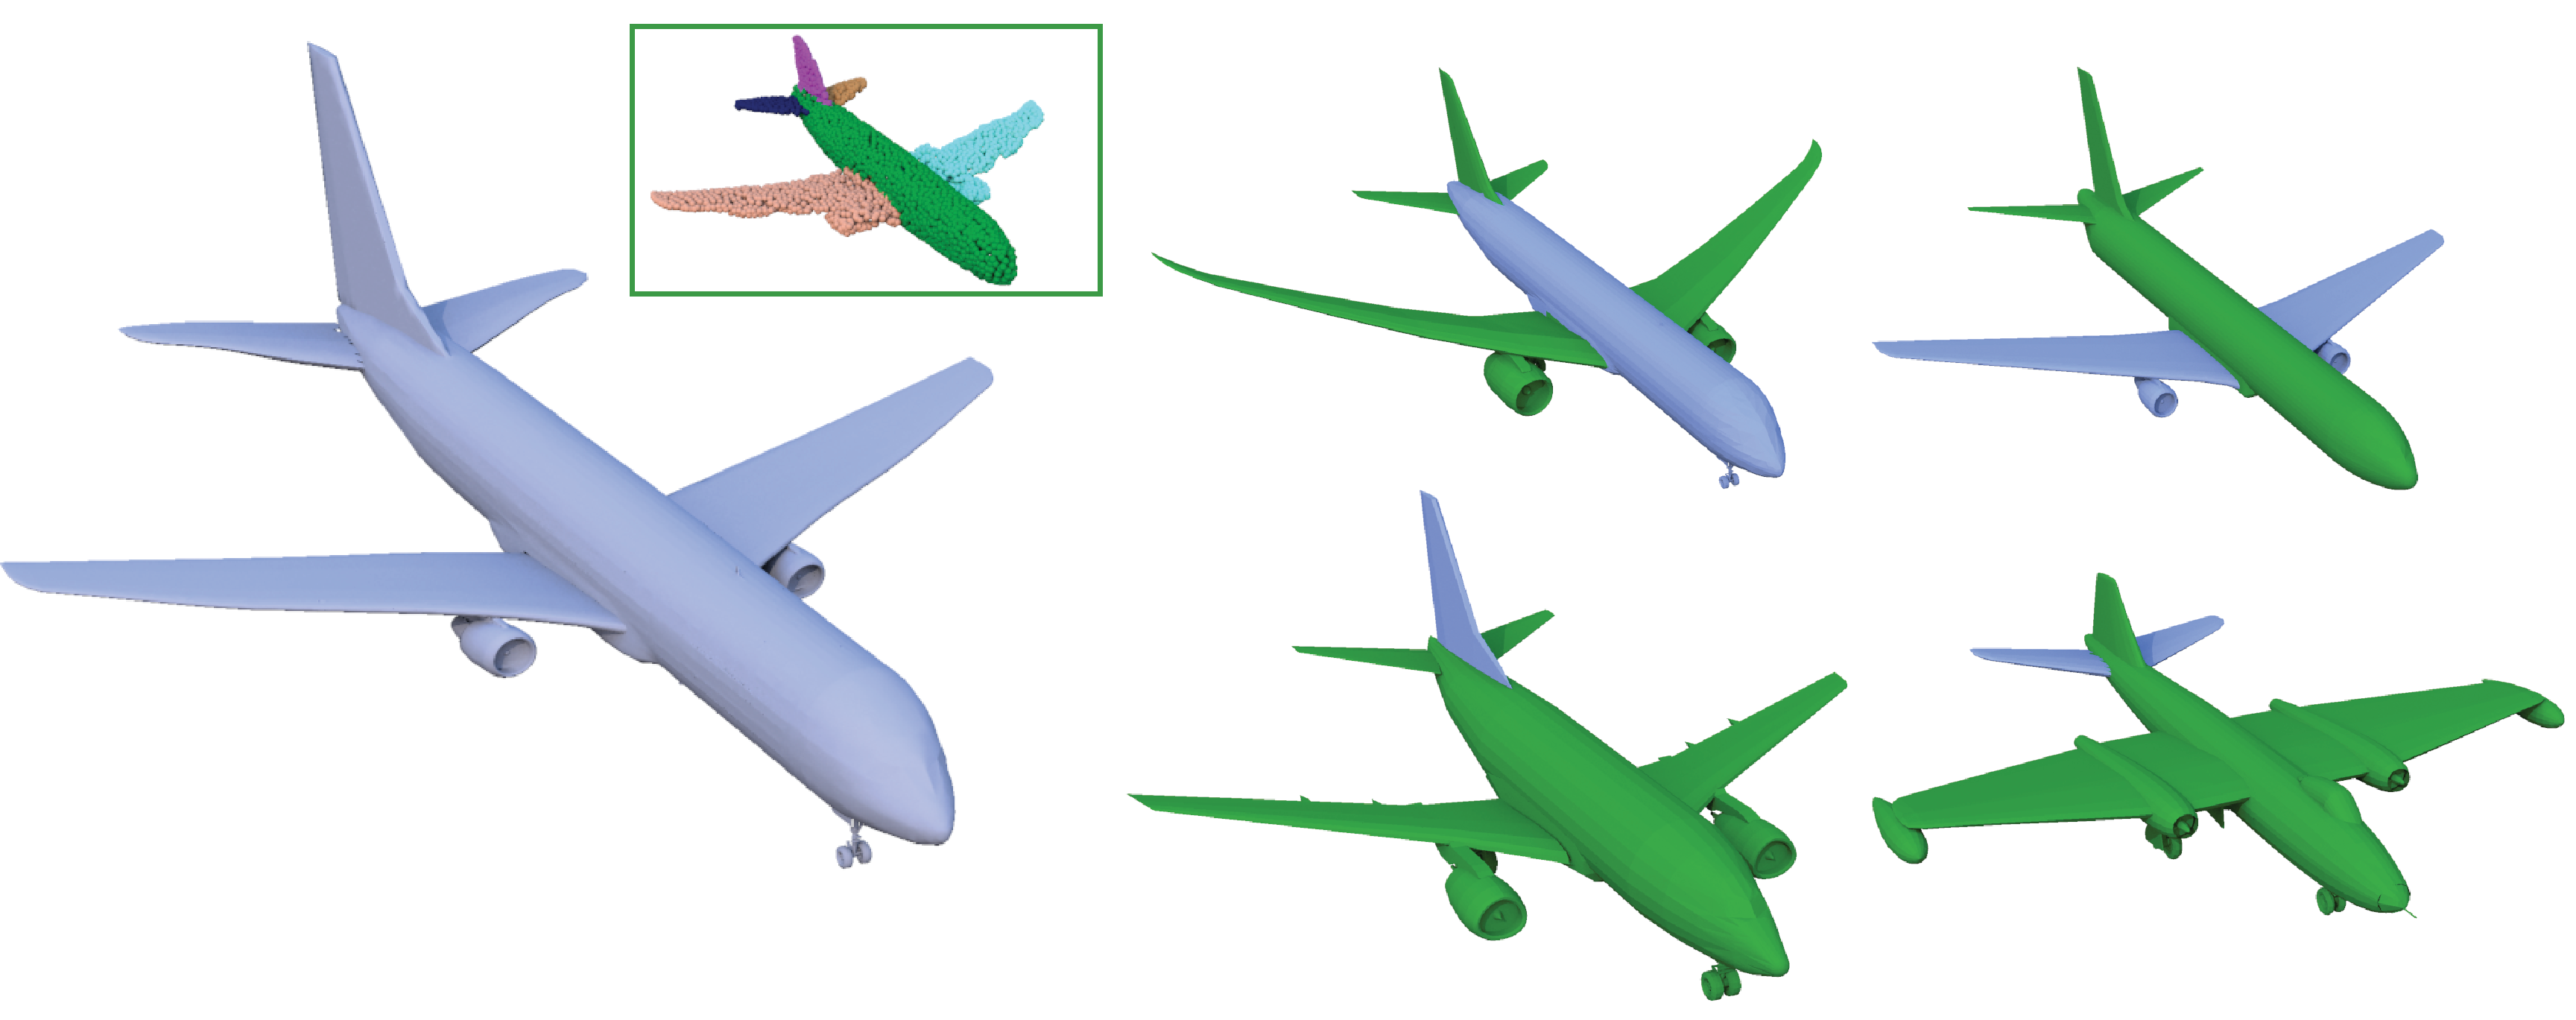
\includegraphics[width=0.83\columnwidth]{figures/synthesis_airplane}
\vskip -1mm
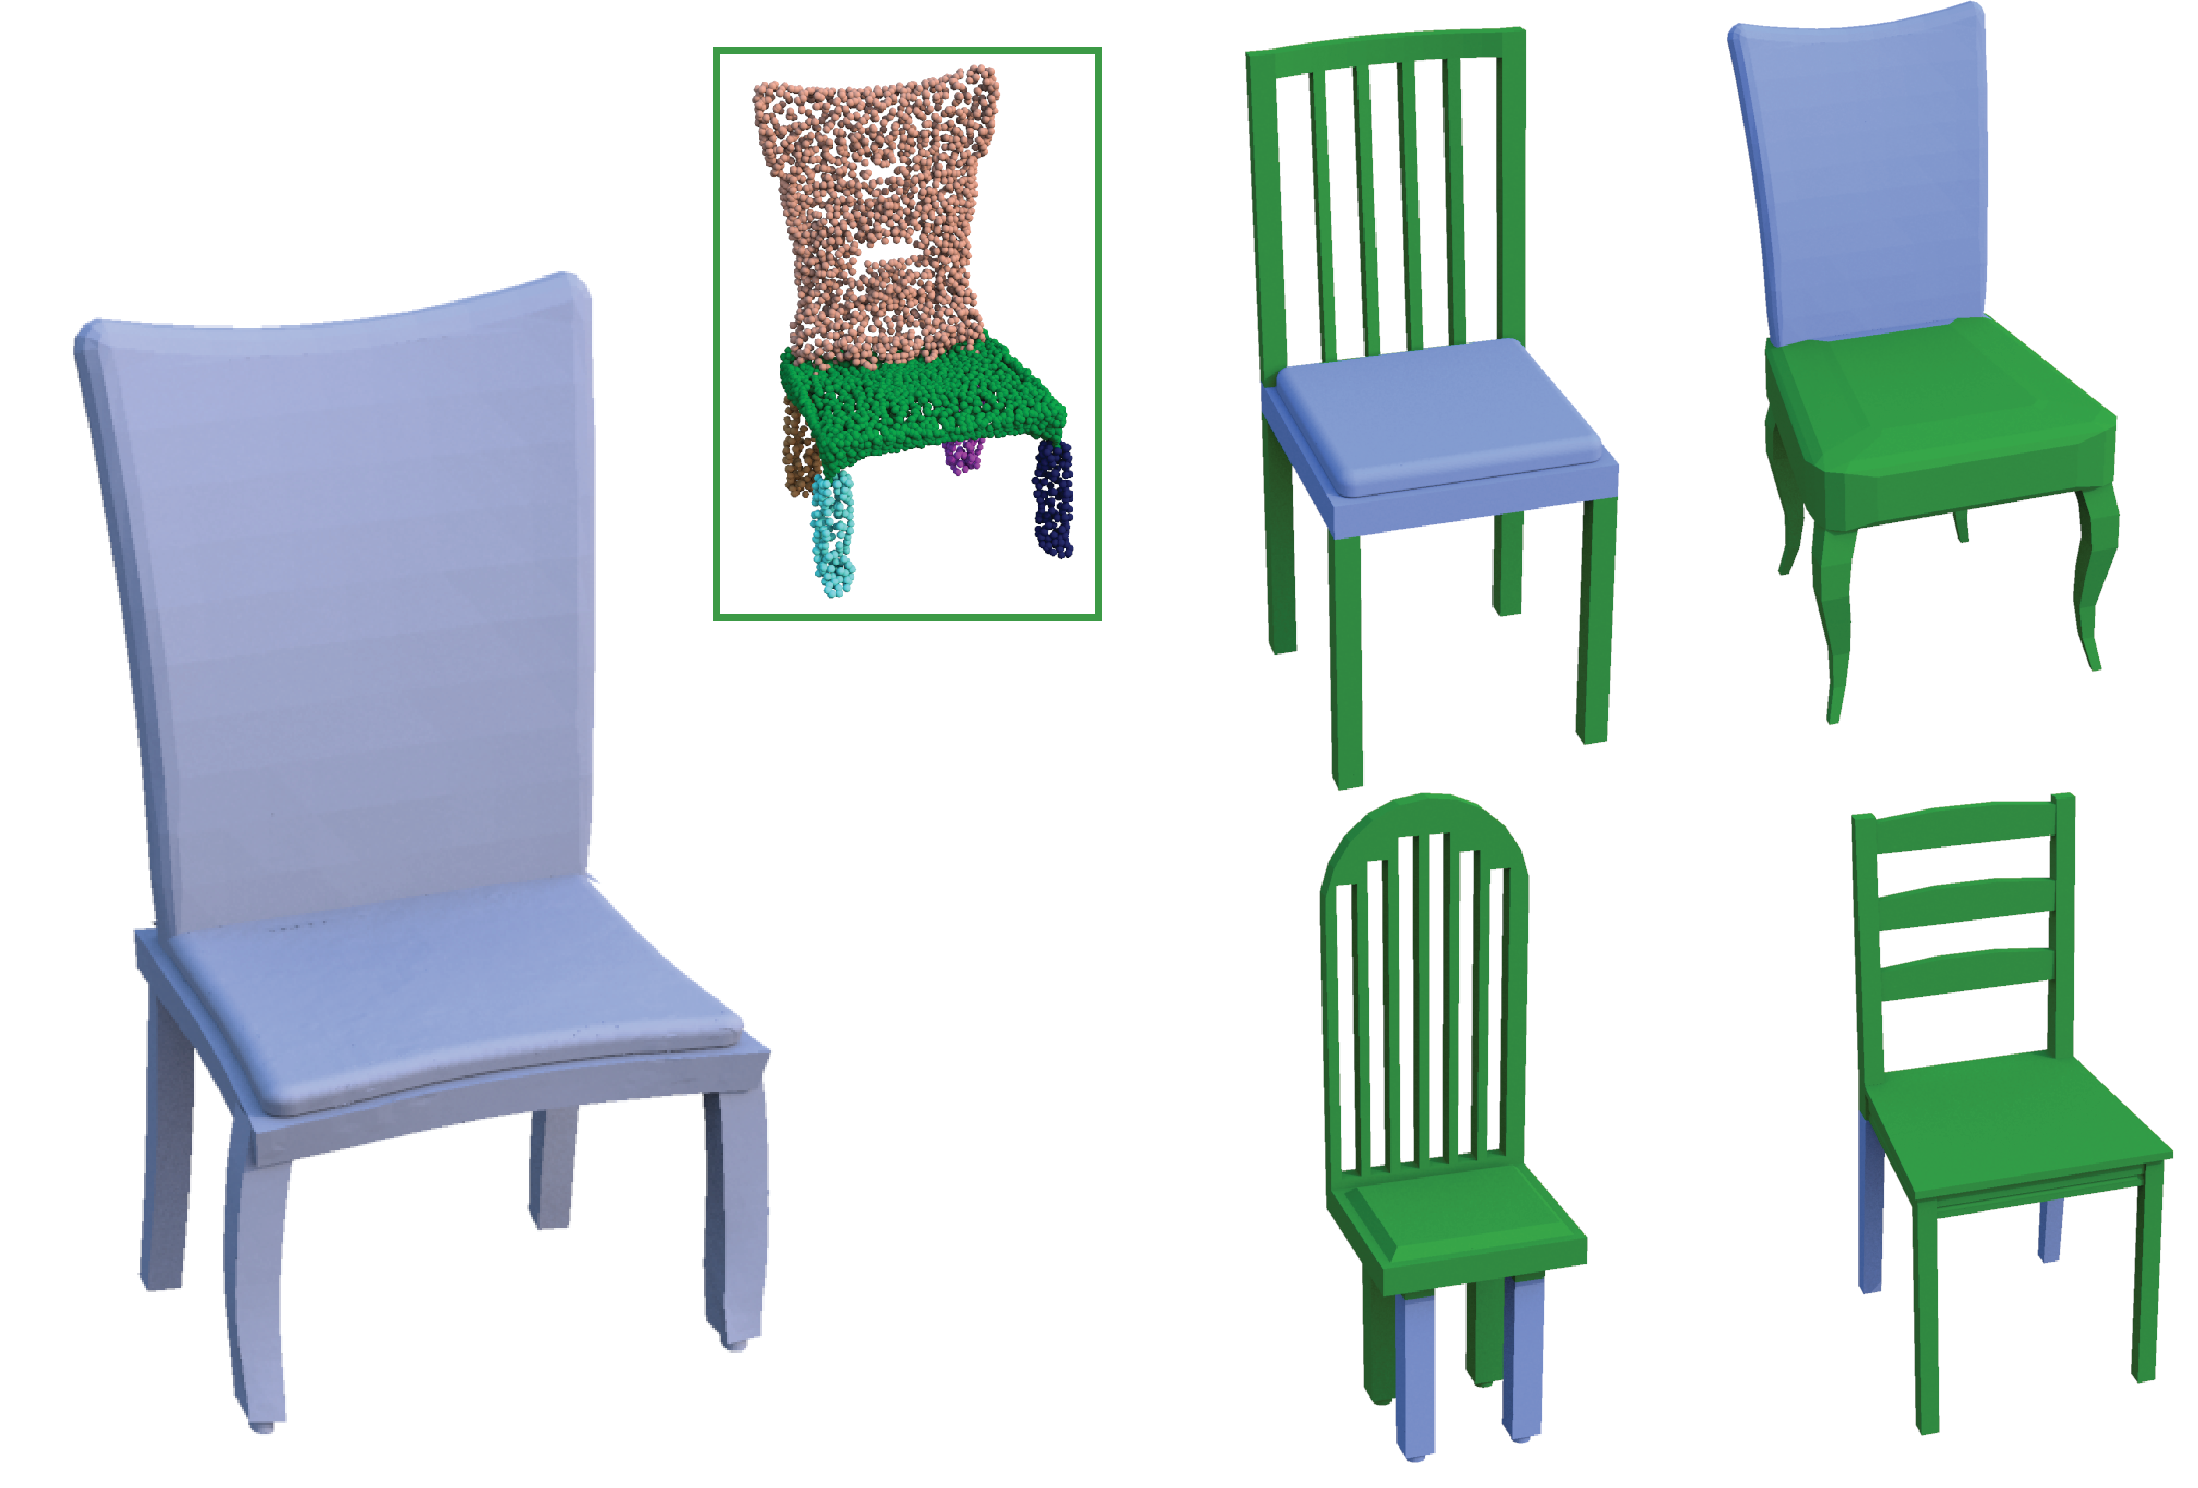
\includegraphics[width=0.83\columnwidth]{figures/synthesis_chair}
\vskip -3mm
\caption{Synthesis of new shapes (left) based on the Beta Shape Machine samples (green box) and embedded deformation on input shape parts (right).}
\vskip -8mm
\label{fig:synthesis_results}
\end{figure}



%%%%%%%%%%%%%%%%%%%%%%%%%%%%%%%%%%%%%%%%%%%%%%%%%%%%%%%%%%%%%%%%%%%%%%%%
% Results
%%%%%%%%%%%%%%%%%%%%%%%%%%%%%%%%%%%%%%%%%%%%%%%%%%%%%%%%%%%%%%%%%%%%%%%%

\vskip -3mm
\section{Results}
\label{sec:results_applications}

\begin{figure*}[t!]
\hskip -3mm
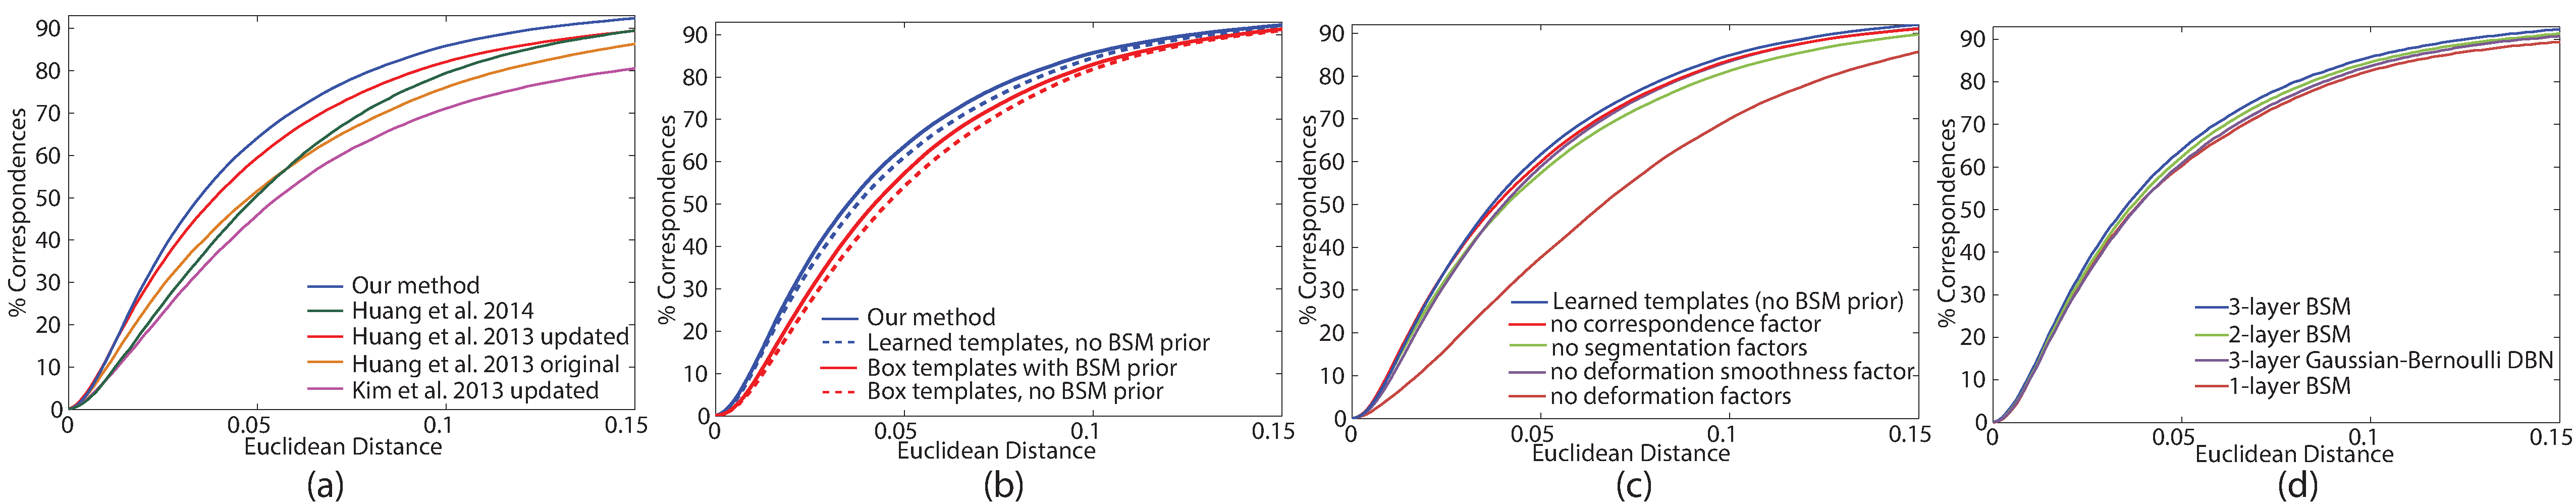
\includegraphics[width=1.03\textwidth]{figures/CORRECTED_correspondence_all.pdf}
\vskip -3mm
\caption{Correspondence accuracy of our method in Kim et al.'s benchmark versus (a) previous approaches, (b) using box templates and skipping the BSM surface prior, (c) skipping factors from the CRF deformation model, (d) versus alternative Deep Boltzmann Machine formulations.}
\vskip -8mm
\label{fig:correspondence_accuracy_all}
\end{figure*}

We now describe the experimental validation of our method for computing semantic point correspondences, shape segmentation, fine-grained classification, and synthesis.

\textbf{Correspondence accuracy.} We evaluated the performance of our method on the recent benchmark provided by Kim et al. \shortcite{Kim13}. We refer to it as BHCP benchmark. The benchmark provides positions of ground-truth points in a collection of $404$ shapes from Trimble Warehouse including bikes, helicopters, chairs and airplanes. We compared our algorithm with previous methods whose authors made their results publically available or agreed to share results with us on the same benchmark: Figure \ref{fig:correspondence_accuracy_all}a demonstrates the performance of our method, the box template fitting method by Kim et al. \shortcite{Kim13}, the local non-rigid registration method by Huang et al. \shortcite{Huang13}, and the functional map network method also by Huang et al \cite{Huang14}. We report the performance of Huang et al.'s method \shortcite{Huang13} based on the originally published results as well as the latest updated results kindly provided by the authors. Following Kim et al.'s protocol, we measure the Euclidean distance error between each provided ground-truth point position and its corresponding point position predicted by the competing methods averaged over all the pairs of shapes in the benchmark. The y-axis demonstrates the fraction of correspondences predicted correctly below a given Euclidean error threshold shown on the x-axis. We stress that all methods are compared using the same protocol evaluated over all the pairs of the shapes contained in the benchmark, as also done in previous work. The performance of our algorithm is reported using the BSM surface prior together with the CRF deformation model. Our \rev{part templates} were initialized based on the co-segmentations provided by Kim et al. (no manual segmentations were used). Our surface prior was learned in a subset of the large datasets used in Kim et al. ($1509$ airplanes, $408$ bikes, $3701$ chairs, $406$ helicopters). We did not use their whole dataset because we excluded shapes whose provided template fitting error according to their method was above the median error value for airplanes and chairs, and above the $90$th percentile for bikes and chairs indicating possible wrong rigid alignment. A few tens of models could also not be downloaded based on the provided original web links. To ensure a fair comparison, we updated the performance of Kim et al. by learning the template parameters in the same subset as ours. Their method had slightly better performance compared to using the original dataset ($0.95\%$ larger fraction of correspondences predicted correctly at distance $0.05$). Huang et al.'s reported experiments and results do not make use of the large datasets, but are based on pairwise alignments and networks within the ground-truth sets of the shapes in the benchmark. Figure \ref{fig:correspondence_accuracy_all}a indicates that our method outperforms the other algorithms. In particular, we note that even if we initialized our method with Kim et al.'s segmentations, the final output of our method is significantly better: $18.2\%$ more correct predictions at $0.05$ distance than Kim et al.'s method. 

We provide images of the corresponding feature points and labeled segmentations for the shapes of our large datasets in the supplementary material as well as Figures \ref{fig:teaser} (left) and \ref{fig:chairs_synthesis} (left). All these results were produced by initializing our method with the co-segmentations provided by Kim et al. (no manual shape segmentation was used). We also provide correspondence accuracy plots for each category separately in the supplementary material. 



%\begin{figure}[t!]
%\centering
%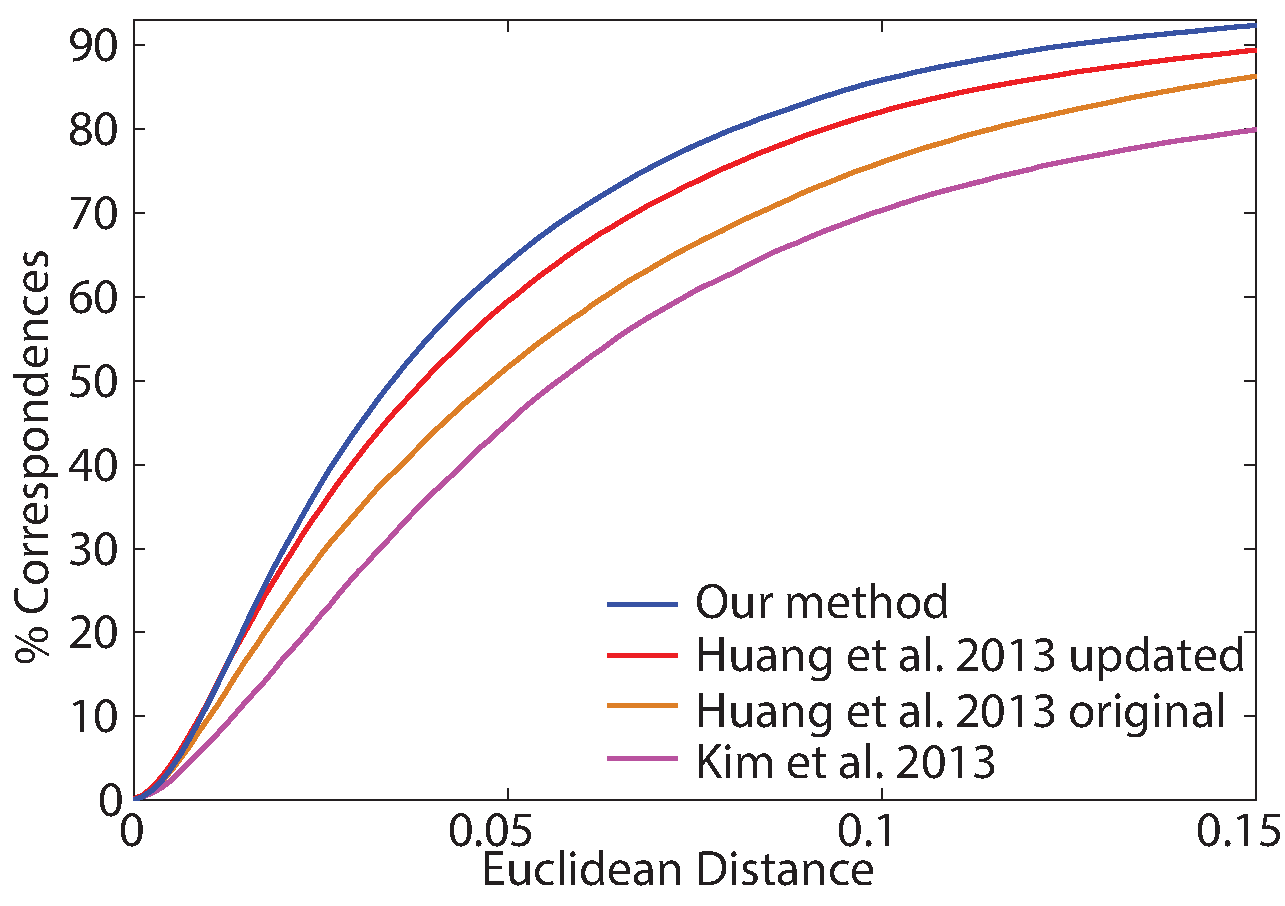
\includegraphics[width=.9\columnwidth]{figures/CORRECTED_correspondence_average.pdf}
%\caption{Correspondence accuracy of our method in Kim et al.'s benchmark compared to previous approaches.}
%\label{fig:correspondence_accuracy_main}
%\end{figure}

\textbf{Alternative formulations.} We now evaluate the performance of our method compared to alternative formulations. First, we show the performance of our method in the case it does not learn \rev{part templates}, but instead uses the same mean-field deformation procedure on the box templates provided by Kim et al. In other words, we deform boxes instead of learned parts. Figure \ref{fig:correspondence_accuracy_all}b shows that the correspondence accuracy is significantly better with the learned \rev{part templates}. In the same plot, we show the performance of the two versions of our method with and without the BSM surface prior. We note that using the BSM prior improves correspondence accuracy either in the case of box or learned part templates. 

%Figure \ref{mf_iterations} demonstrates the improvement in the correspondence accuracy for each mean-field iteration for learning the \rev{part templates}. After about $8$ iterations, mean-field converges, and there is no more significant improvement. 

%\begin{figure}[t]
%\centering
%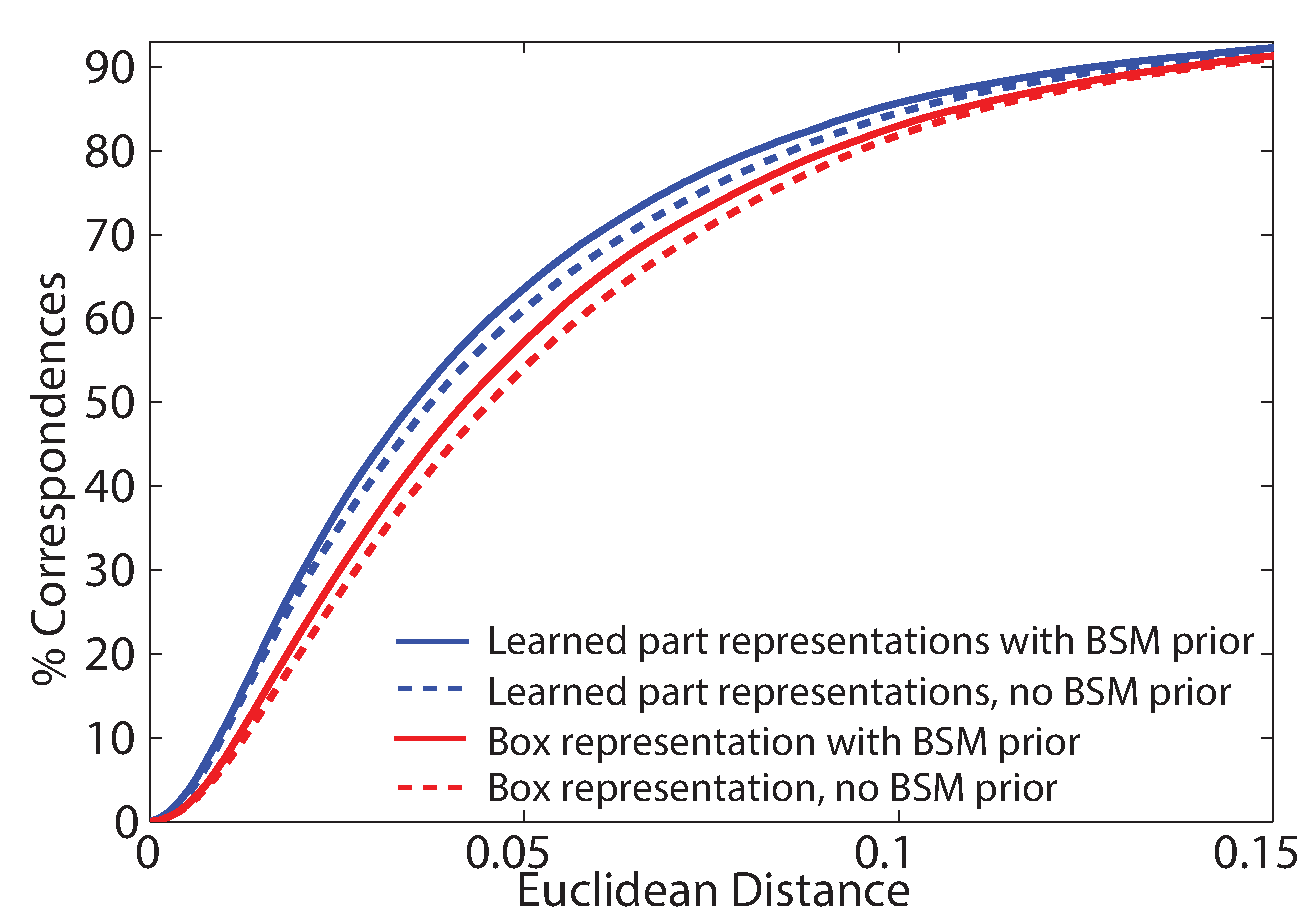
\includegraphics[width=.9\columnwidth]{figures/CORRECTED_correspondence_accuracy_different_models.pdf}
%\caption{Correspondence accuracy of our method in Kim et al.'s benchmark versus using deformed box representations or skipping the BSM surface prior.}
%\label{fig:correspondence_accuracy2}
%\end{figure}

%\begin{figure}[t]
%\centering 
%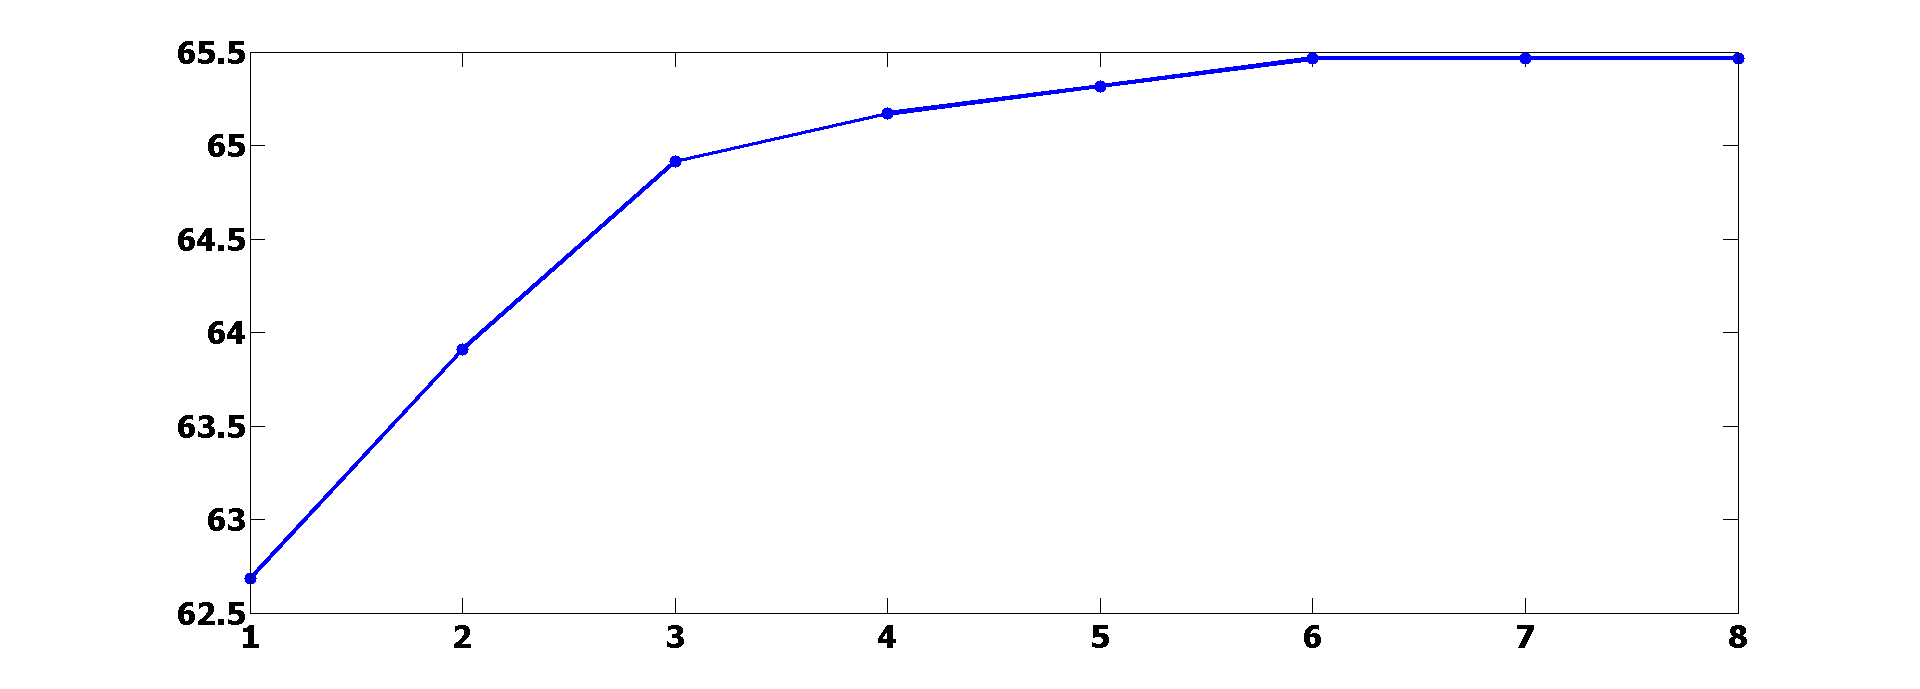
\includegraphics[width=1.0\columnwidth]{figures/accuracy_learned}
%\caption{ Fraction of correspondences predicted correctly below $0.05$ error threshold versus running more mean-field %iterations for learning the \rev{part templates} (variables $\bY$).  }
%\label{fig:mf_iterations}
%\end{figure}
 
We also evaluate the performance of our method by testing the contribution of the different factors used in the CRF deformation model. Figure \ref{fig:correspondence_accuracy_all}c shows the correspondence accuracy in the same benchmark by using all factors in our model (top curve), without using the unary deformation, deformation smoothness, correspondence or segmentation factors. For all these alternative models, we do not include the BSM prior to factor out its influence. As shown in the plot, all factors contribute to the improvement of the performance. In particular, skipping the deformation or segmentation parts of the model cause a noticeable performance drop. 

Finally, we evaluate the performance of our method by using different formulations of the surface prior. Figure \ref{fig:correspondence_accuracy_all}d demonstrates the correspondence accuracy of our three-layer BSM model (original model), versus a two-layer and a single-layer BSM model. In addition, we include a comparison with a Deep Boltzmann Machine that uses Gaussian instead of Beta distributions (Gaussian-Bernoulli DBM) using three layers and the same training procedure. Our three-layer BSM model provides the best performance. Using more layers did not yield any significant improvement based on our datasets.

%\begin{figure}[t]
%\centering
%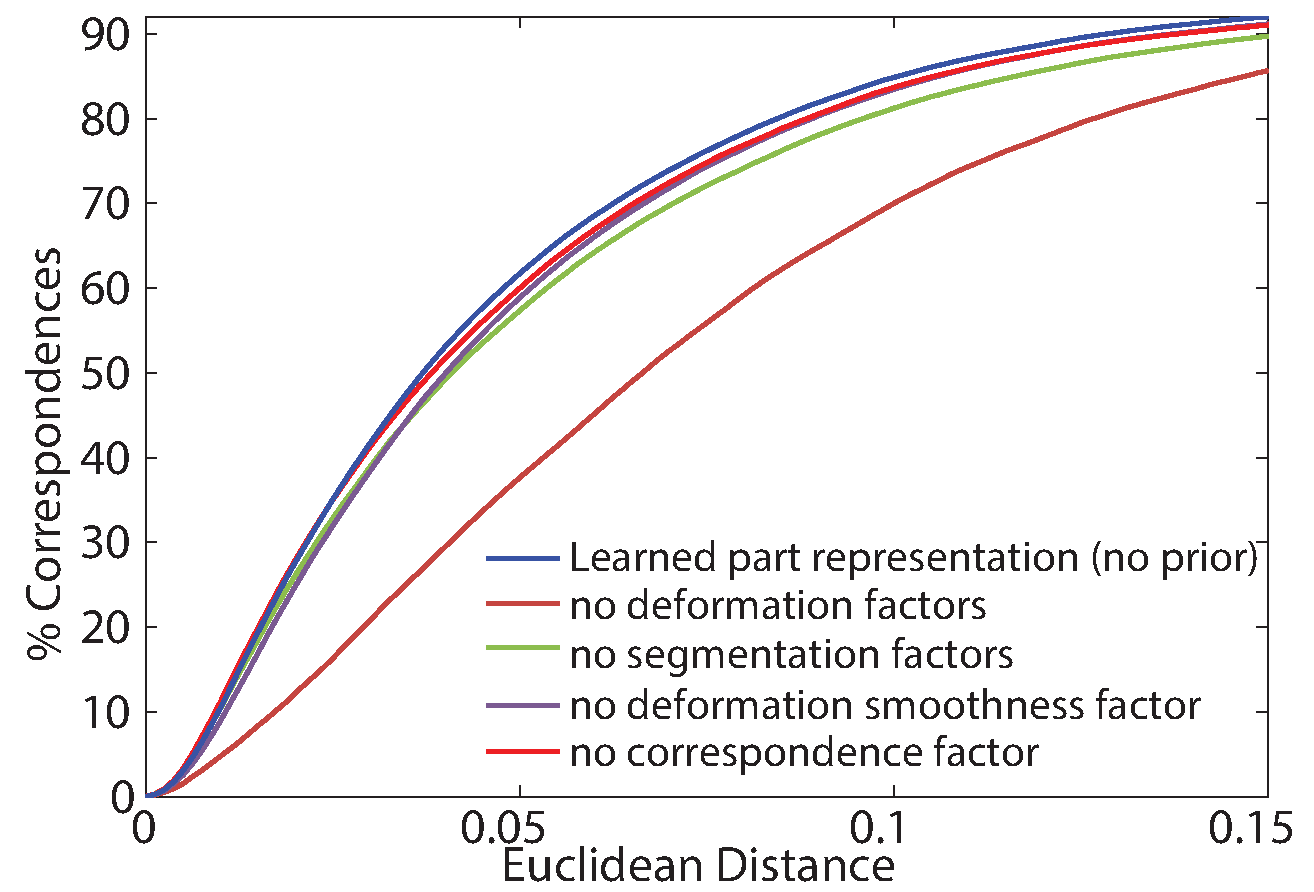
\includegraphics[width=.9\columnwidth]{figures/CORRECTED_correspondence_factor_diff.pdf}
%\caption{Correspondence accuracy of our method in Kim et al.'s benchmark versus skipping different factors from the CRF model.}
%\label{fig:correspondence_accuracy3}
%\end{figure}

\vskip -2mm
\begin{table}[h]
\centering
\begin{tabular}{|@{}c@{}|@{}c@{}|@{}c@{}|@{}c@{}|@{}c@{}|}
\hline
 Category           & Num.            & \,Kim et al.\, & Our          & Num. \\
 (Dataset)          & \,shapes\,      & \,(our init.)\,  & \,method\, & \,groups\, \\  
\hline  
 Bikes (BHCP)        & 100   & 76.8 & 82.3 & 2 \\
 Chairs (BHCP)       & 100   & 81.2 & 86.8 & 2\\
 Helicopters (BHCP)  & 100   & 80.1 & 87.4 & 1 \\
 Planes (BHCP)       & 104   & 85.8 & 89.6 & 2 \\
\hline  
 Lamps (COSEG)      & 20    & 95.2 & 96.5 & 1 \\
 Chairs (COSEG)     & 20    & 96.7 & 98.5& 1 \\
 Vase (COSEG)       & 28    & 81.3 & 83.3& 2 \\
 Quadrupeds (COSEG) & 20    & 86.9 & 87.9& 3 \\
 Guitars (COSEG)    & 44    & 88.5 & 89.2 & 1 \\
 Goblets (COSEG)    & 12    & 97.6 & 98.2 & 1\\
 Candelabra (COSEG) & 20    & 82.4 & 87.8 & 3\\
 Large Chairs (COSEG) & 400 & 91.2 & 92.0 & 5 \\
 Large Vases (COSEG)  & 300 & 85.6 & 83.0 & 5 \\
\hline 
\end{tabular}
\vskip -1mm
\caption{Labeling accuracy of our method versus Kim et al.}
\label{table:results_coseg}
\vskip -2mm
\end{table}

\begin{figure*}[t]
\centering
\includegraphics[width=0.95\textwidth]{figures/teaser_chair}
\vskip -2mm
\caption{Left: Shape correspondences and segmentations for chairs. Right: Synthesis of new chairs}
\label{fig:chairs_synthesis}
\vskip -8mm
\end{figure*}

\textbf{Segmentation accuracy.} We now report the performance of our method for shape segmentation. We evaluated the segmentation performance on the COSEG dataset \cite{Wang12} and a new dataset we created: we labeled the parts of the $404$ shapes used in the BHCP correspondences benchmark. We provide images of the ground-truth segmentations in the supplementary material. We compared our method with Kim et al.'s segmentations in these datasets based on the publically available code and data. These are the same segmentations that we used to initialize our method (no manual segmentations were used). For both methods, we evaluate the labeling accuracy by measuring the fraction of faces for which the part label predicted by our method agrees with the ground-truth label. Since our method provides segmentation at a point cloud level, we transfer the part labels from points to faces using the same graph cuts as in Kim et al. Table \ref{table:results_coseg} shows that our method yields better labeling performance. The difference is noticeable in complex shapes, such as helicopters, airplanes, bikes and candelabra.  The same table reports the number of clusters (groups) used in our model. We note that our method could be initialized with any other unsupervised technique. This table indicates that our method tends to improve the segmentations it was initialized with. 

\textbf{Fine-grained classification.} \rev{The uppermost layer of the BSM model can be used to produce a compact, class-specific shape descriptor. We demonstrate its use in the context of fine-grained classification. For this purpose, we labeled the BHCP benchmark shapes with fine-grained class labels: we categorized airplanes into commercial jets, fighter jets, propeller aircraft and UAVs, chairs into benches, armchairs, side and swivel chairs, and bikes into bicycles, tricycles and motorbikes. We compute activation probabilities in the uppermost layer through mean-field inference given each input shape, and used those as  descriptors. Using $10$ training examples per class, and a single nearest neighbor classification scheme based on $L^1$ norm distance, the rest of the shapes were classified with accuracy $92\%$, $94\%$, $96.5\%$ for airplanes, chairs, and bikes respectively. Descriptors, results, training and test splits are included in the supplementary material.}

\textbf{Shape synthesis.} Figure \ref{fig:teaser}(right) and \ref{fig:chairs_synthesis}(right) demonstrates synthesized chairs and airplanes using samples from the BSM model trained on these large collections. Our shape synthesis procedure makes use of the shape parts segmented by our method in these collections. However, not all shapes are segmented perfectly: even if the labeling accuracy of our method is high as demonstrated above, minor errors along segmentation boundaries (e.g., mislabeled individual faces crossing boundaries) cause visual artifacts when shapes are assembled from these segmented parts. Such errors are common in graph cuts. Corrections would require re-meshing or other low-level mesh operations. We instead manually flagged $25\%$ of airplanes and $40\%$ of chairs with imperfect segmentation boundaries. These were excluded during the nearest neighbors procedure for selecting parts given the BSM samples. We still believe that the amount of human supervision for this process is much smaller compared to previous generative models \cite{Kalogerakis12} that required manually specified shape segmentations for at least half or the whole input collections. We also conducted a perceptual evaluation of our synthesized shapes with $31$ volunteers recruited through Amazon Mechanical Turk. Our user study indicates that the shapes produced by our model were seen as plausible as the training shapes of the input collections. We include the user study details and results in the supplementary material. We also provide images of $500$ synthesized airplanes and chairs in the supplementary material.   

\textbf{Running times.} The mean-field procedure (Algorithm \ref{algorithm}) requires $6$ hours for our largest dataset (3K chairs). Learning the BSM model requires $45$ hours on the same dataset. Running times are reported on a E5-2697 v2 processor. Running times scale linearly with the dataset size.

\vspace{-2mm}



%%%% OLD TABLE
%\begin{table}[h]
%\hskip -3mm
%\footnotesize
%\begin{tabular}{|@{}c@{}|@{}c@{}|@{}c@{}|@{}c@{}|@{}c@{}|@{}c@{}|}
%\hline
% Category & Num.       & \cite{Huang14}\,   & \cite{Kim13}\, & Our          & Num. \\
% (Dataset)& \,shapes\, & \,(F-maps)\,       & \,(our init.)\,  & \,method\, & \,groups\, \\  
%\hline  
% Bikes (BHCP)         & 100   & N/A           & 76.8 & \textbf{82.3} & 2 \\
% Chairs (BHCP)        & 100   & N/A           & 81.2 & \textbf{86.8} & 2 \\
% Helicopters (BHCP)   & 100   & N/A           & 80.1 & \textbf{87.4} & 1 \\
% Planes (BHCP)        & 104   & N/A           & 85.8 & \textbf{89.6} & 2 \\
%\hline  
% Lamps (COSEG)        & 20    & 96.1          & 95.2 & \textbf{96.5} & 1 \\
% Chairs (COSEG)       & 20    & 93.9          & 96.7 & \textbf{98.5} & 1 \\
% Vase (COSEG)         & 28    & \textbf{88.5} & 81.3 & 83.3          & 2 \\
% Quadrupeds (COSEG)   & 20    & 74.8          & 86.9 & \textbf{87.9} & 3 \\
% Guitars (COSEG)      & 44    & \textbf{93.4} & 88.5 & 89.2          & 1 \\
% Goblets (COSEG)      & 12    & 91.2          & 97.6 & \textbf{98.2} & 1 \\
% Candelabra (COSEG)   & 20    & \textbf{93.1} & 82.4 & 87.8          & 3 \\
% Large Chairs (COSEG) & 400   & \textbf{98.1} & 91.2 & 92.0          & 5 \\
% Large Vases (COSEG)  & 300   & \textbf{94.3} & 85.6 & 83.0          & 5 \\
%\hline 
%\end{tabular}
%\vskip -2mm
%\caption{Labeling accuracy of our method versus Kim et al.}
%\label{table:results_coseg}
%\vskip -2mm
%\end{table}




%%%%%%%%%%%%%%%%%%%%%%%%%%%%%%%%%%%%%%%%%%%%%%%%%%%%%%%%%%%%%%%%%%%%%%%%
% Conclusion
%%%%%%%%%%%%%%%%%%%%%%%%%%%%%%%%%%%%%%%%%%%%%%%%%%%%%%%%%%%%%%%%%%%%%%%%

\vskip -3mm
\section{Limitations and Discussion}
\label{sec:limitations_discussion}

\rev{Our paper described a method for joint shape analysis and synthesis in a shape collection: our method learns \rev{part templates}, computes shape correspondence and part segmentations, generates new shape surface variations, and yields shape descriptors for fine-grained classification. Our method represents an early attempt in this area, thus there are several limitations to our method and many exciting directions for future work.} First, our method is greedy in nature. Our method relies on approximate inference for both the CRF deformation and the BSM generative model. Learning relies on approximate techniques. As a result, the sampled point clouds are not smooth and noiseless. We used conservative deformations of parts from the input collection to factor out the noise and preserve surface detail during shape synthesis. Assembling shapes from parts suffers from various limitations: adjacent parts are not always connected in a plausible manner, segmentation artifacts affect the quality of the produced shapes, topology changes are not supported. Instead of re-using parts from the input collection, it would be more desirable to extend our generative model with layers that produce denser point clouds. In this case, the denser point clouds could be used as input to surface reconstruction techniques to create new shapes entirely from scratch. However, the computational cost for learning such generative model with dense output would be much higher. From this aspect, it would be interesting to explore more efficient learning techniques in the future. Our \rev{part template} learning procedure relies on provided initial rigid shape alignments and segmentations, which can sometimes be incorrect. \rev{It would be better to fully exploit the power of our probabilistic model to perform rigid alignment. Deep learning architectures could be used to estimate initial segmentations and correspondences.} \rev{The learned shape descriptor could improve the shape grouping}. Finally, the variability of the synthesized shapes seems somewhat limited. Fruitful directions include investigating deeper architectures, better sampling strategies, and matching \rev{ templates} with multiple symmetric parts if such exist in the input shapes. 

\vspace{-2mm}

\paragraph*{Acknowledgements.} 
Kalogerakis gratefully acknowledges support from NSF (CHS-1422441).
We thank Qi-xing Huang and Vladimir Kim for sharing data from their methods.
We thank Siddhartha Chaudhuri and anonymous reviewers for valuable comments. 
We thank Szymon Rusinkiewicz for distributing the trimesh2 library. 

\vspace{-1mm}


\vskip -3mm

%%%%%%%%%%%%%%%%%%%%%%%%%%%%%%%%%%%%%%%%%%%%%%%%%%%%%%%%%%%%%%%%%%%%%%%%
% Appendix
%%%%%%%%%%%%%%%%%%%%%%%%%%%%%%%%%%%%%%%%%%%%%%%%%%%%%%%%%%%%%%%%%%%%%%%%
%\appendix
%\section{Mean-field inference equations}
\label{sec:mean-field-appendix}

According to the mean-field approximation theory \cite{Koller09}, given a probability distribution $P$ defined over a set of variables $X_1, X_2, ..., X_V$, we can approximate it with a simpler distribution $Q$, expressed as a product of individual distributions over each variable, such that the KL-divergence of $P$ from $Q$ is minimized: 

\begin{align*}
KL(Q \mid \mid P) = \sum\limits_{X_1}\sum\limits_{X_2}...\sum\limits_{X_V} Q(X_1, X_2, ..., X_V) \cdot \ln \frac{ Q(X_1, X_2, ..., X_V) } { P(X_1, X_2, ..., X_V) }
\end{align*}
In the case of continuous variables, the above sums are replaced with integrals over their value space. Suppose that the original distribution $P$ is defined  as a product of factors:
\begin{align*}
P(X_1, X_2, ..., X_V) = \frac{1}{Z} \prod\limits_{s=1...S} \phi_s(\bD_s)
\end{align*}
where $\bD_s$ is a subset of the random variables (called scope) for each factor $s$ in the distribution $P$, and $Z$ is a normalization constant. 

Minimizing the KL-divergence  of $P$ from $Q$ yields the following mean-field updates for each variable $X_v$ ($v=1...V$):
\begin{align*}
Q(X_v) = \frac{1}{Z_v} \exp \bigg\{ \sum\limits_s \sum\limits_{\bD_s-\{X_v\}} Q( \bD_s-\{X_v\} ) \ln \phi_s(\bD_s) \bigg\}
\end{align*}
where $Z_v=\sum\limits_{X_v} Q(X_v)$ is a normalization constant for this distribution (the sum is replaced with the integral over the value space of $X_v$ if this is a continuous variable), and $\bD_s-\{X_v\}$ is the subset of the random variables for the factor $s$ excluding the variable $X_v$. 

Below we specialize the above update formula for each of our variable in our probabilistic model. 


\subsection{Deformation variables}

The mean-field update for each deformation variables is the following:

\begin{align*}
Q(\bD_{t,k}) \propto \exp\bigg\{ & -0.5 \sum\limits_p Q(U_{t,p} = k) (\bD_{t,k} - \bX_{t,p})^T \Sigma_1^{-1} (\bD_{t,k} - \bX_{t,p}) \\
& -0.5 \sum\limits_{k' \in N(k)} (\bD_{t,k} - \bmu_{t,k,k'})^T \Sigma_2^{-1}(\bD_{t,k} - \bmu_{t,k,k'} )  \bigg\}
\end{align*}
where $\mN(k)$ includes all neighboring points $k'$ of point $k$ on the \rev{part template} (see main text of the paper) and $\bmu_{t,k}$ is a 3D vector defined as follows:
\begin{align*}
\bmu_{t,k,k'} = \Ex_Q[\bD_{t,k'}] + ( \Ex_Q[\bY_{k}] - \Ex_Q[\bY_{k'}] ) )
\end{align*}

We note that the above distribution is a product of Gaussians; when re-normalized, the distribution is equivalent to a Gaussian with the following expectation, or mean, which we use in other updates:

\begin{align}
\Ex_Q[\bD_{t,k}]  = & ( \sum\limits_p Q(U_{t,p} = k) \Sigma_1^{-1}  + \sum\limits_{k' \in N(k)}\Sigma_2^{-1} )^{-1}  \nonumber  \\
&\cdot ( \sum\limits_p Q(U_{t,p} = k) \Sigma_1^{-1} \bX_{t,p} + \sum\limits_{k' \in N(k)}\Sigma_2^{-1} \bmu_{t,k,k'}  )
\label{eqn:D}
\end{align}

The above formula indicates that the most likely deformed position of a point on a \rev{part template} is a weighted average of its associated points on the input surface as well as its neighbors. The weights are controlled by the covariance matrices $\Sigma_1$ and $\Sigma_2$ as well as the degree of association between the \rev{part template} point and each input surface point, given by $Q(U_{t,p}=k)$. The covariance matrix of the above distribution is forced to be diagonal (see next section); its diagonal elements tend to increase when the input surface points have weak associations with the \rev{part template} point, as indicated by the following formula:

\begin{align*}
Cov_Q[\bD_{t,k}]  = ( \sum\limits_p Q(U_{t,p} = k) \Sigma_1^{-1}  + \sum\limits_{k' \in N(k)}\Sigma_2^{-1} )^{-1}
\end{align*}

Computing the above expectation and covariance for each variable $\bD_{t,k}$ involving summing over every surface point $p$ on the input shape $t$. This is computationally too expensive. Practically in our implementation, we find the $100$ nearest input surface points for each \rev{part template} point $k$, and we also find the $20$ nearest \rev{part template} points for each input surface point $p$. For each \rev{template} point $k$, we always keep indices to its $100$ nearest surface points as well as the surface points whose nearest points include that \rev{template} point $k$. Instead of summing over all the surface points of each input shape, for each \rev{template} point $k$ we sum over its abovementioned indices to surface point only. For the rest of the surface points, the distribution values  $Q(U_{t,p}=k)$ are practically negligible and are skipped in the above summations.


\subsection{Part template variables}

For each \rev{part template} point $\bY_k$, the mean-field update is given by:

\begin{align*}
& Q(\bY_k) \propto \exp\bigg\{ -.5(\bY_k - \bmu_k )^T \Sigma_2^{-1} ( \bY_k -  \bmu_k )  \bigg\}
\end{align*}
where $\bmu_k$ is the mean, or expectation (3D vector), defined as follows:
\begin{align*}
\bmu_k = \Ex_Q[\bY_{k}] = \frac{1}{|\mN(k)|} \sum\limits_{k'} \big( \Ex_Q[\bY_{k'}] + \frac{1}{T}\sum\limits_t(\Ex_Q[\bD_{t,k}] - \Ex_Q[\bD_{t,k'}]) \big)
\end{align*}
and $\mN(k)$ includes all neighboring points $k'$ of point $k$ on the \rev{part template}, $T$ is the number of input shapes. The covariance matrix for the above distribution is given by $\Sigma_2$. 

\subsection{Point correspondence variables}

The mean-field update for the latent variables $U_{t,p}$ yields a categorical distribution computed as follows:

\begin{align*}
Q(U_{t,p} = k) \propto \exp\bigg\{ & - 0.5(\Ex_Q[\bD_{t,k}] - \bX_{t,p})^T \Sigma_1^{-1} (\Ex_Q[\bD_{t,k}] - \bX_{t,p}) \\ 
& -0.5 Tr( \Sigma_1^{-1} \cdot Cov_Q[\bD_{t,k}] ) \\
& -0.5(\bff_{k} - \bff_{t,p})^T \Sigma_3^{-1} (\bff_{k} - \bff_{t,p})  - \ln\epsilon \cdot Q(S_{t,p} = label(k)) \bigg\}
\end{align*}

where $Tr( \Sigma_1^{-1} \cdot Cov_Q[\bD_{t,k}] )$ represents the matrix trace, $\epsilon$ is a small constant discussed in the main text of the paper. For computational efficiency reasons, we avoid computing the above distribution for all pairs of \rev{part template} and input surface points. As in the case of the updates for the deformation variables,  we keep indices to input surface point positions that are nearest neighbors to \rev{part template} points and vice versa. We compute the above distributions only for pairs between these neighboring points. For the rest of the pairs, we set $Q(U_{t,p}=k) = 0$.

\subsection{Segmentation variables}

The mean-field update for the variables $S_{t,p}$ also yields a categorical distribution:

\begin{align*}
Q(S_{t,p} = l) \propto \exp\bigg\{ & \sum\limits_k Q(U_{t,p} = k) [label(k) \ne l] \ln\epsilon \\
& + \sum\limits_{p' \in N(p)} \sum\limits_{l' \ne l} Q(S_{t,p'} = l' ) \ln( 1.0 - \Phi ) \\
& + \sum\limits_{p' \in N(p)} Q(S_{t,p'} = l ) \ln( \Phi ) \bigg\} \\
\end{align*}

where $N(p)$ is the neighborhood of the input surface point used for segmentation (see main text for more details), $Phi$ evaluates feature differences between neighboring surface points (see main text for its definition). The binary indicator function $[label(k) \ne l]$ is $1$ if the expression in brackets holds, otherwise it is $0$. 
%(i.e., the evaluated label $l$ of the input surface point is different than the label of its corresponding \rev{part template} point)

\section{Covariance matrix updates}

The covariance matrices of our factors are updated as follows: 

\begin{align*}
\Sigma_1 & = \frac{1}{Z_1} \sum\limits_{t,k,p \in \mN(k)} Q(U_{t,p} = k) (\Ex_Q[\bD_{t,k}] - \bX_{t,p}) (\Ex_Q[\bD_{t,k}] - \bX_{t,p})^T \\
\end{align*}
\begin{align*}
\Sigma_2 = \frac{1}{Z_2} \sum\limits_{t,k,k' \in N(k)} & ( (\Ex_Q[\bD_{t,k}] - \Ex_Q[\bD_{t,k'}]) - (\Ex_Q[\bY_k] - \Ex_Q[\bY_{k'}]) ) \cdot \\
& \cdot (\Ex_Q[\bD_{t,k}] - \Ex_Q[\bD_{t,k'}] - (\Ex_Q[\bY_k] - \Ex_Q[\bY_{k'}]) )^T
\end{align*}
\begin{align*}
\Sigma_3 = \frac{1}{Z_3}\sum\limits_{t,k,p \in \mN(k)}  Q(U_{t,p} = k) (\bff_k - \bff_{t,p}) (\bff_k - \bff_{t,p})^T 
\end{align*}
\begin{align*}
\Sigma_5 = \frac{1}{Z_5} \sum\limits_{t,p,p' \in N(p)} ( \bff_{t,p} - \bff_{t,p'}) ( \bff_{t,p} - \bff_{t,p'})^T \\
\end{align*}

where $Z_1=Z_3=\sum\limits_{t,k,p \in \mN(k)} Q(U_{t,p} = k)$, $Z_2=\sum\limits_{t,k,k' \in N(k)} 1$, $Z_5=\sum\limits_{t,p,p' \in N(p)} 1$. The computed covariance matrices are forced to be diagonal i.e., in the above computations only the diagonal elements of the covariance matrices are taken into account, while the rest of the elements are set to $0$. 


\section{Contrastive divergence}

Contrastive divergence iterates over the following three steps in our implementation: variational (mean-field) inference, stochastic approximation (or sampling), and parameter updates. We discuss the steps in detail below. 

\textbf{Variational inference step.} 
Our deformation model yields expectations over deformed point positions of the \rev{part templates} based on Equation \ref{eqn:D}. For each deformed point, we find the surface point that is closest to its expected position. Let $D_{k,\tau}[t]$ the observed surface position of point $k$ for an input shape $t$. The subscript $\tau$ takes values $1$, $2$, or $3$ that correspond to the $x-$,$y-$,$z-$ coordinate of the point respectively. Let $E_{k}[t]$ represents the observed existence of a point $k$ (binary variable) also inferred by our deformation model. Given all observed point positions  $\bD[t]$ and existences $\bE[t]$ per shape $t$, we perform bottom-up mean-field inference on the binary hidden nodes according to the following equations in the following order:

\begin{align*}
Q( H_m^{(1)} = 1 | \bD[t], \bE[t] ) =
\sigma \bigg( w_{m, 0} & + \sum\limits_{k \in \mN_m,\tau} (  a_{k,\tau,m} - c_{k,\tau,m} ) \ln(D_{k,\tau}[t]) E_k[t] \\
& + \sum\limits_{k \in \mN_m,\tau} (  b_{k,\tau,m} - d_{k,\tau,m} ) \ln(1 - D_{k,\tau}[t]) E_k[t] \\
& +  \sum\limits_{n} w_{m, n} Q( H_n^{(2)} = 1 | \bD[t], \bE[t] ) \bigg)
\end{align*}
\begin{align*}
Q( H_n^{(2)} = 1 | \bD[t], \bE[t] ) = \sigma \bigg( w_{n, 0} & + 
 \sum\limits_{m} w_{m, n} Q( H_m^{(1)} = 1 | \bD[t], \bE[t] ) \\
& + \sum\limits_{o} w_{n, o} Q( H_o^{(3)} = 1 | \bD[t], \bE[t] ) \bigg)
\end{align*}
\begin{align*}
Q( H_o^{(3)} = 1 | \bD[t], \bE[t] ) = \sigma \bigg( w_{o, 0} + \sum\limits_{n} w_{n, o} Q( H_n^{(2)} = 1 | \bD[t], \bE[t] ) \bigg)
\end{align*}

where $\sigma(\cdot)$ represents the sigmoid function, $\mN_m$ is the set of the observed variables each hidden node (variable) $H_m^{(1)}$ is connected to. The mean-field updates for $H_m^{(1)}$ involve a weighted summation over the observed variables $\bD[t]$ per part, which can be thought of as a convolutional scheme per part. We perform $3$ mean-field iterations alternating the updates over the above hidden nodes. During the first iteration, we initialize $Q( H_n^{(2)} = 1 )=0$ and $Q( H_o^{(3)} = 1 ) = 0$ for each hidden node $n$ and $o$. 

\textbf{Stochastic approximation}. This step begins by sampling the binary hidden nodes of the top layer for each training shape $t$. Sampling is performed according to the inferred distributions $Q( H_o^{(3)} = 1 | \bD[t], \bE[t] )$ of the previous step. Let $H_o^{(3)}[t']$ the resulting sampled $0/1$ values. Then we perform top-down mean-field inference on the binary hidden nodes of the other layers as well as the visible layer: 

\begin{align*}
Q( H_n^{(2)} = 1 | \bE[t], \bH^{(3)}[t'] ) = \sigma \bigg( w_{n, 0} & + 
    \sum\limits_{m} w_{m, n} Q( H_m^{(1)} = 1 | \bE[t], \bH^{(3)}[t'] ) \\
& + \sum\limits_{o} w_{n, o} H_o^{(3)}[t'] \bigg)
\end{align*}
\begin{align*}
Q( H_m^{(1)} = 1 | \bE[t], \bH^{(3)}[t'] ) =
\sigma \bigg( w_{m, 0} & + \sum\limits_{k \in \mN_m,\tau} (  a_{k,\tau,m} - c_{k,\tau,m} ) \ln(D_{k,\tau}[t']) E_k[t] \\
& + \sum\limits_{k \in \mN_m,\tau} (  b_{k,\tau,m} - d_{k,\tau,m} ) \ln(1 - D_{k,\tau}[t']) E_k[t] \\
& + \sum\limits_{n} w_{m, n} Q( H_n^{(2)} = 1 | \bE[t], \bH^{(3)}[t'] ) \bigg)
\end{align*}
\begin{align*}
& Q( D_{k,\tau} | \bE[t], \bH^{(3)}[t'] ) \propto \\
& D_{k,\tau} ^{ (a_{k,\tau,0}-1) + \sum\limits_{m \in \mN_k} a_{k,\tau,m} Q( H_m^{(1)} = 1 | \bE[t], \bH^{(3)}[t'] ) 
+ \sum\limits_{m \in \mN_k} c_{k,\tau,m} (1-Q( H_m^{(1)} = 1 | \bE[t], \bH^{(3)}[t'] ))} \\
&  (1-D_{k,\tau}) ^{ (b_{k,\tau,0}-1) + \sum\limits_{m \in \mN_k} b_{k,\tau,m} Q( H_m^{(1)} = 1 | \bE[t], \bH^{(3)}[t'] ) 
+ \sum\limits_{m \in \mN_k} d_{k,\tau,m} (1-Q( H_m^{(1)} = 1 | \bE[t], \bH^{(3)}[t'] ))}
\end{align*}
where $D_{k,\tau}[t']$ in the above mean-field updates is set to be the expectation of the above Beta distribution and $\mN_k$ is the set of the hidden variables each observed node (variable) $D_{k,\tau}$ is connected to. We note that sampling all the variables in the model caused contrastive divergence not to converge, thus we instead used expectations of the above distributions instead. As in the previous step, we performed $3$ iterations alternating over the above mean-field updates. During the first iteration, we skip the terms involving $D_{k,\tau}[t']$ during the inference of the hidden nodes of the first layer. At the second and third iteration, we infer distributions for the hidden layers as follows:
\begin{align*}
Q( H_o^{(3)} = 1 | \bD[t'], \bE[t] ) = \sigma \bigg( w_{o, 0} + \sum\limits_{n} w_{n, o} Q( H_n^{(2)} = 1 | \bD[t'], \bE[t] ) \bigg)
\end{align*}
\begin{align*}
Q( H_n^{(2)} = 1 | \bD[t'], \bE[t] ) = \sigma \bigg( w_{n, 0} & + 
    \sum\limits_{m} w_{m, n} Q( H_m^{(1)} = 1 | \bD[t'], \bE[t] ) \\
& + \sum\limits_{o} w_{n, o} Q( H_o^{(3)} = 1 | \bD[t'], \bE[t] ) \bigg)
\end{align*}
\begin{align*}
Q( H_m^{(1)} = 1 | \bD[t'], \bE[t]] ) =
\sigma \bigg( w_{m, 0} & + \sum\limits_{k \in \mN_m,\tau} (  a_{k,\tau,m} - c_{k,\tau,m} ) \ln(D_{k,\tau}[t']) E_k[t] \\
& + \sum\limits_{k \in \mN_m,\tau} (  b_{k,\tau,m} - d_{k,\tau,m} ) \ln(1 - D_{k,\tau}[t']) E_k[t] \\
& + \sum\limits_{n} w_{m, n} Q( H_n^{(2)} = 1 | \bD[t'], \bE[t] ) \bigg)
\end{align*}


\textbf{Parameter updates}. The parameters of the model are updated with project gradient ascent according to the expectations over the final distributions computed in the previous two steps and the observed data. We list the parameter updates below. We note that $sgn(\cdot)$ used below denotes the sign function, $\nu$ is the iteration number (or epoch), $\eta$ is the learning rate, $\mu$ is the momentum rate. The learning rate is set to $0.001$ initially, and is multiplied by a factor $0.9$ when at the previous epoch the reconstruction error $\sum_{t,k,\tau} |D_{k,\tau}[t] E_k[t] -  D_{k,\tau}[t'] E_k[t] |$ increases, and it is multiplied by a factor $1.1$ when the reconstruction error decreases. The momentum rate is progressively increased from $0.5$ towards $1.0$ asymptotically during training.

\begin{align*}
a_{k,\tau,0} = max( a_{k,\tau,0} + \Delta a_{k,\tau,0}[\nu], 0 ) \textrm{\,\,\,\,, where}
\end{align*}
\begin{align*}
\Delta a_{k,\tau,0}[\nu] & = \mu \cdot \Delta a_{k,\tau,0}[\nu-1] + \eta \frac{1}{T}\sum\limits_t \bigg( \ln(D_{k,\tau}[t]) - \ln(D_{k,\tau}[t']) \bigg) \\
& - \eta \lambda_1 \sum\limits_{k' \in \mN_k} sgn( a_{k,\tau,0} - a_{k',\tau,0} ) - \eta \lambda_2 sgn( a_{k,\tau,0} ) \\
\end{align*}

\begin{align*}
b_{k,\tau,0} = max( b_{k,\tau,0} + \Delta b_{k,\tau,0}[\nu], 0 ) \textrm{\,\,\,\,, where} \\
\end{align*}
\begin{align*}
\Delta b_{k,\tau,0}[\nu] & = \mu \cdot \Delta b_{k,\tau,0}[\nu-1] + \eta \frac{1}{T}\sum\limits_t  \bigg( \ln(1-D_{k,\tau}[t]) - \ln(1-D_{k,\tau}[t']) \bigg) \\
& - \eta \lambda_1 \sum\limits_{k' \in \mN_k} sgn( b_{k,\tau,0} - b_{k',\tau,0} ) - \eta \lambda_2 sgn( b_{k,\tau,0} )  \\
\end{align*}

\begin{align*}
a_{k,\tau,m} = max( a_{k,\tau,m} + \Delta a_{k,\tau,m}[\nu], 0) \textrm{\,\,\,\,, where}
\end{align*}
\begin{align*}
\Delta a_{k,\tau,m}[\nu] & = \mu \cdot \Delta a_{k,\tau,m}[\nu-1] + \eta \frac{1}{T}\sum\limits_t \bigg( \ln(D_{k,\tau}[t]) Q( H_m^{(1)} = 1 | \bD[t], \bE[t] ) \\
     								  				  &-\ln(D_{k,\tau}[t']) Q( H_m^{(1)} = 1 | \bD[t'], \bE[t] ) \bigg) \\
& - \eta \lambda_1 \sum\limits_{k' \in \mN_k} sgn( a_{k,\tau,m} - a_{k',\tau,m} ) - \eta \lambda_2 sgn( a_{k,\tau,m} ) \\
\end{align*}

\begin{align*}
b_{k,\tau,m} = max( b_{k,\tau,m} + \Delta b_{k,\tau,m}[\nu], 0) \textrm{\,\,\,\,, where}
\end{align*}
\begin{align*}
\Delta b_{k,\tau,m}[\nu] &= \mu \cdot \Delta b_{k,\tau,m}[\nu-1] + \eta \frac{1}{T}\sum\limits_t  \bigg( \ln(1-D_{k,\tau}[t]) Q( H_m^{(1)} = 1 | \bD[t], \bE[t] ) \\
     								  				  &-\ln(1-D_{k,\tau}[t']) Q( H_m^{(1)} = 1 | \bD[t'], \bE[t] ) \bigg) \\
& - \eta \lambda_1 \sum\limits_{k' \in \mN_k} sgn( b_{k,\tau,m} - b_{k',\tau,m} ) - \eta \lambda_2 sgn( b_{k,\tau,m} )  \\
\end{align*}

\begin{align*}
c_{k,\tau,m} = max( c_{k,\tau,m} + \Delta c_{k,\tau,m}[\nu], 0) \textrm{\,\,\,\,, where}
\end{align*}
\begin{align*}
\Delta c_{k,\tau,m}[\nu] &= \mu \cdot \Delta c_{k,\tau,m}[\nu-1] + \eta \frac{1}{T}\sum\limits_t  \bigg( \ln(D_{k,\tau}[t]) (1-Q( H_m^{(1)} = 1 | \bD[t], \bE[t] ) \\
     								  				  &-\ln(D_{k,\tau}[t']) (1-Q( H_m^{(1)} = 1 | \bD[t'], \bE[t] ) \bigg) \\
& - \eta \lambda_1 \sum\limits_{k' \in \mN_k} sgn( c_{k,\tau,m} - c_{k',\tau,m} ) - \eta \lambda_2 sgn( c_{k,\tau,m} )  \\
\end{align*}

\begin{align*}
d_{k,\tau,m} = max( d_{k,\tau,m} + \Delta d_{k,\tau,m}[\nu], 0) \textrm{\,\,\,\,, where}
\end{align*}
\begin{align*}
\Delta d_{k,\tau,m}[\nu] &= \mu \cdot \Delta d_{k,\tau,m}[\nu-1] + \eta\frac{1}{T}\sum\limits_t  \bigg( \ln(1-D_{k,\tau}[t]) (1-Q( H_m^{(1)} = 1 | \bD[t], \bE[t] ) \\     								  				  &-\ln(1-D_{k,\tau}[t']) (1-Q( H_m^{(1)} = 1 | \bD[t'], \bE[t] ) \bigg) \\
& - \eta \lambda_1 \sum\limits_{k' \in \mN_k} sgn( d_{k,\tau,m} - d_{k',\tau,m} ) -\eta \lambda_2 sgn( d_{k,\tau,m} )  \\
\end{align*}

\begin{align*}
w_{m, 0} = w_{m, 0} + \Delta w_{m, 0}[\nu]  \textrm{\,\,\,\,, where}
\end{align*}
\begin{align*}
\Delta w_{m, 0}[\nu] &= \mu \cdot \Delta w_{m, 0}[\nu-1] + \eta \frac{1}{T}\sum\limits_t  \bigg( Q( H_m^{(1)} = 1 | \bD[t], \bE[t] ) \\
& - Q( H_m^{(1)} = 1 | \bD[t'], \bE[t] ) \bigg) \\
& - \eta \lambda_2 sgn( w_{m, 0} )  \\
\end{align*}

\begin{align*}
w_{n, 0} = w_{n, 0} + \Delta w_{n, 0}[\nu] \textrm{\,\,\,\,, where}
\end{align*}
\begin{align*}
\Delta w_{n, 0}[\nu] &= \mu \cdot \Delta w_{n, 0}[\nu-1] + \eta \frac{1}{T}\sum\limits_t  \bigg( Q( H_n^{(2)} = 1 | \bD[t], \bE[t] ) \\
& - Q( H_n^{(2)} = 1 | \bD[t'], \bE[t] ) \bigg)  \\
& - \eta \lambda_2 sgn( w_{n, 0} ) \\
\end{align*}

\begin{align*}
w_{o, 0} = w_{o, 0} + \Delta w_{o, 0}[\nu] \textrm{\,\,\,\,, where}
\end{align*}
\begin{align*}
\Delta w_{o, 0}[\nu] &= \mu \cdot \Delta w_{o, 0}[\nu-1]  + \eta \frac{1}{T}\sum\limits_t  \bigg( Q( H_o^{(3)} = 1 | \bD[t], \bE[t] ) \\
& - Q( H_o^{(3)} = 1 | \bD[t'], \bE[t]) \bigg) \\
& - \eta \lambda_2 sgn( w_{o, 0} ) \\
\end{align*}


\begin{align*}
w_{m, n} = w_{m, n} + \Delta w_{m, n}[\nu] \textrm{\,\,\,\,, where}
\end{align*}
\begin{align*}
\Delta w_{m, n}[\nu] & = \mu \cdot  \Delta w_{m, n}[\nu-1]  + \eta \frac{1}{T}\sum\limits_t  \bigg( Q( H_m^{(1)} = 1 | \bD[t], \bE[t] ) Q( H_n^{(2)} = 1 | \bD[t], \bE[t] )\\
										   & - Q( H_m^{(1)} = 1 | \bD[t'], \bE[t] ) Q( H_n^{(2)} = 1 | \bD[t'], \bE[t]) \bigg)  \\
										   & - \eta \lambda_2 sgn( w_{m, n} ) \\
\end{align*}


\begin{align*}
w_{n, o} = w_{n, o} + \Delta w_{n, o}[\nu]  \textrm{\,\,\,\,, where}
\end{align*}
\begin{align*}
\Delta w_{n, o}[\nu] &= \mu \cdot \Delta w_{n, o}[\nu-1] + \eta \frac{1}{T}\sum\limits_t  \bigg( Q( H_n^{(2)} = 1 | \bD[t], \bE[t] ) Q( H_o^{(3)} = 1 | \bD[t], \bE[t] ) \\
										   & - Q( H_n^{(2)} = 1 | \bD[t'], \bE[t]) Q( H_o^{(3)} = 1 | \bD[t'], \bE[t]) \bigg) \\
										   & - \eta \lambda_2 sgn( w_{n, o} )  \\
\end{align*}



\subsection{Parameter updates for the structure part of the BSM}
To learn the parameters $w_{k,0}$, $w_{k,r}$, $w_{r,0}$ involving the variables $\bE$ and $\bG$ of the BSM part modeling the shape structure, we similarly perform contrastive divergence with the following steps:

\textbf{Inference.}  Given the observed point existences $\bE[t]$, we infer the following distribution over the latent variables $\bG$ (we note that this is exact inference): 

\begin{align*}
Q( G_r = 1 | \bE[t] ) = \sigma(  w_{r, 0} + \sum\limits_{k} w_{k, r} E_k[t]  )
\end{align*}

\textbf{Sampling.} We sample the binary latent variables $\bG$ according to the inferred distribution $Q( G_r=1 | \bE[t] )$. Let $G_r[t']$ the resulting sampled $0/1$ values. We perform inference for the existence variables as follows:

\begin{align*}
Q( E_k = 1 | \bG[t'] ) = \sigma(  w_{k, 0} + \sum\limits_{r} w_{k, r} G_r[t']  )
\end{align*}

and repeat for the latent variables:

\begin{align*}
Q( G_r = 1 | \bG[t'] ) = \sigma(  w_{r, 0} + \sum\limits_{k} w_{k, r} Q( E_k = 1 | \bG[t'] ) )
\end{align*}

 
\textbf{Parameter updates} The parameters of the structure part of the BSM are updated as follows:


\begin{align*}
w_{k, 0} = w_{k, 0} + \Delta w_{k, 0}[\nu] \textrm{\,\,\,\,, where}
\end{align*}
\begin{align*}
\Delta w_{k, 0}[\nu] &= \mu \cdot \Delta w_{k, 0}[\nu-1]  + \eta \frac{1}{T}\sum\limits_t  \bigg( E_k[t] - Q( E_k = 1 | \bG[t'] ) \bigg) \\
& - \eta \lambda_1 \sum\limits_{k' \in \mN_k} sgn( w_{k, 0} - w_{k', 0} ) - \eta \lambda_2 sgn( w_{k, 0} )  \\
\end{align*}

\begin{align*}
w_{r, 0} = w_{r, 0} + \Delta w_{r, 0}[\nu]   \textrm{\,\,\,\,, where}
\end{align*}
\begin{align*}
\Delta w_{r, 0}[\nu] &= \mu \cdot \Delta w_{r, 0}[\nu-1] + \eta \frac{1}{T}\sum\limits_t  \bigg( Q( G_r = 1 | \bE[t] ) - Q( G_r =1 | \bG[t'] ) \bigg) \\
&  - \eta \lambda_2 sgn( w_{r, 0} ) 
\end{align*}


\begin{align*}
w_{k, r} = w_{k, r} + \Delta w_{k, r}[\nu] \textrm{\,\,\,\,, where}
\end{align*}
\begin{align*}
\Delta w_{k, r}[\nu] &= \mu \cdot \Delta w_{k, r}[\nu-1] + \eta \frac{1}{T}\sum\limits_t  \bigg( E_k[t] Q( G_r = 1 | \bE[t] ) \\ 
& - Q( E_k = 1 | \bG[t'] )Q( G_r =1 | \bG[t'] ) \bigg) \\
&  - \eta \lambda_1 \sum\limits_{k' \in \mN_k} sgn( w_{k, r} - w_{k', r} ) - \eta \lambda_2 sgn(w_{k, r})  \\
\end{align*}



%%%%%%%%%%%%%%%%%%%%%%%%%%%%%%%%%%%%%%%%%%%%%%%%%%%%%%%%%%%%%%%%%%%%%%%%
% Acknowledgements 
%%%%%%%%%%%%%%%%%%%%%%%%%%%%%%%%%%%%%%%%%%%%%%%%%%%%%%%%%%%%%%%%%%%%%%%%

%\begin{acks}
%We are grateful to.... 
%\end{acks}

%-------------------------------------------------------------------------

\bibliographystyle{eg-alpha-doi}
\bibliography{bbbm}

%-------------------------------------------------------------------------


\end{document}
